% Gerar um texto com o conteúdo da apresentação
% \documentclass[class=article]{beamer}
\documentclass[10pt,aspectratio=1610,lualatex]{beamer}
\mode<presentation>
%\documentclass[dvips]{beamer}
%\documentclass[notes]{beamer}
 \usepackage{beamerbaserequires}
 \usepackage{beamerbaseoptions}
% \usepackage{beamerbasearticle}
\usepackage{appendixnumberbeamer}
\usepackage[portuguese,brazil,brazilian]{babel}
\usepackage[utf8]{luainputenc}
%\usepackage{xunicode}% 
%\usepackage{xltxtra}%
%\usepackage{metalogo}%
%\usepackage{xkeyval}%
%\usepackage{polyglossia}
%\usepackage{lmodern}
\usepackage{ifluatex}
%\usepackage{times}
\usepackage{ae}
%\usepackage{helvet}
\usepackage{bm}
\usepackage[no-math]{fontspec}
\usepackage{pifont}
\usepackage{FiraSans}
\usepackage{amsfonts}
\usepackage{amsmath}
% \usepackage{unicode-math}
\usepackage{amsthm}
%\usepackage{cmbright}
%\usepackage{cmbright}
\usepackage[T1]{fontenc}
\usepackage{amssymb}
\usepackage{color}
\usepackage{animate}
\usepackage{multimedia}
\usepackage{media9}
\usepackage{beamerthemesplit}
\usepackage{booktabs}
\usepackage{parskip}
\usepackage{microtype}
\usepackage{setspace}
\usepackage{pdflscape}
\usepackage{hyperref}
% \hypersetup{
%   colorlinks=true,    % false: boxed links; true: colored links
%   linkcolor=blue,     % color of internal links
%   citecolor=blue,     % color of links to bibliography
%   filecolor=magenta,  % color of file links
%   urlcolor=blue,
%   bookmarksdepth=4
%   pdftitle={Mostra PG 2017}, 
%   pdfauthor={Sabrina Tigik Ferr\~ao},
%   pdfsubject={Mostra PG 2017},
%   pdfkeywords={plasma}{plasma kinetic theory}{collisions}
%   {quasilinear theory}{weak turbulence theory} 
% }
\usepackage{url}
\usepackage{graphicx}
\usepackage{pdfpages} 
\usepackage{caption}
\usepackage{ifxetex}
\usepackage{xspace}
\usepackage{xcolor}
% short arrows
\usepackage{stmaryrd}
\usepackage{units}
\usepackage{calc}
\usepackage{tikz}
\usepackage{etoolbox}
\usepackage[scale=2]{ccicons}
\usepackage{pgffor}
\usepackage{pgfplots}
\usepackage{pgfopts}
\usepackage{pgfplotsthemetol}
\usepgfplotslibrary{dateplot}
\pgfplotsset{compat=newest}
%\usefonttheme{professionalfonts}
% \useinnertheme{metropolis}
% \useoutertheme{metropolis}
% \usefonttheme{metropolis}

% \useoutertheme{progressbar}
% \useinnertheme{progressbar}
% \usefonttheme{progressbar}

% \usetheme{AnnArbor}
% \usetheme{Antibes}
% \usetheme{Arkyenell}
% \usetheme{bars}
% \usetheme{Berlin}
% \usetheme{BerlinFU}
% \usetheme{Bergen}
% \usetheme{Berkeley}
% \usetheme{Boadilla}
% \usetheme{boxes}
% \usetheme{CambridgeUS}
% \usetheme{classic}
% \usetheme{Copenhagen}
% \usetheme{Cuerna}
% \usetheme{Darmstadt}
% \usetheme{default}
% \usetheme{DetlevCM}
% \usetheme{Dresden}
% \usetheme{epyt}
% \usetheme{EastLansing}
% \usetheme{Frankfurt}
% \usetheme{Goettingen}
% \usetheme{Hannover}
% \usetheme{Ilmenau}
% \usetheme{Jacobs}
% \usetheme{JLTree}
% \usetheme{JuanLesPins}
% \usetheme{lankton-keynote}
% \usetheme{lined}
% \usetheme{Luebeck}
% \usetheme{Madrid}
% \usetheme{Malmoe}
% \usetheme{Marburg}
\usetheme[progressbar=frametitle,numbering=fraction,sectionpage=progressbar,subsectionpage=progressbar]{metropolis}
% \usetheme{Montpellier}
% \usetheme{PaloAlto}
% \usetheme{PhnomPenh}
% \usetheme{Pittsburgh}
% \usetheme{progressbar}
% \usetheme{Rochester}
% \usetheme{shadow}
% \usetheme{sidebar}
% \usetheme{Singapore}
% \usetheme{split}
% \usetheme{Szeged}
% \usetheme{TorinoTh} %não funciona direito
% \usetheme{tree}
% \usetheme{Warsaw}

% \setbeamercovered{transparent}

%% Color themes
% \usecolortheme{Arkyenell}
% \usecolortheme{beaver}
% \usecolortheme{bluesimplex}
% \usecolortheme{bluedawn}
% \usecolortheme{crane}
% \usecolortheme{dolphin}
% \usecolortheme{dove}
% \usecolortheme{ETII} % BR colors
% \usecolortheme{fly}
% \usecolortheme{goeagles}
% \usecolortheme{hohenheim}
% \usecolortheme{lily}
% \usecolortheme{MedStarColors}
% \usecolortheme{metropolis}
% \usecolortheme{monarca}
% \usecolortheme{orchid}
% \usecolortheme{penn}
  \usecolortheme{progressbar}
% \usecolortheme[snowy]{owl}
% \usecolortheme{rose}
% \usecolortheme{seagull}
% \usecolortheme{seahorse}
% \usecolortheme{solarized}
% \usecolortheme{spruce}
% \usecolortheme{torinoth} 
% \usecolortheme{whale}
% \usecolortheme{wolverine}
% %% dark color themes %%
% \usecolortheme[overlystylish]{albatross}
% \usecolortheme{albatross}
% \usecolortheme{beetle}
% \usecolortheme[cautious]{owl}
% \usecolortheme{cormorant}
% \usecolortheme{frigatebird}
% \usecolortheme{magpie}
% \usecolortheme[dark]{solarized}

%% Fonte padrão do LaTeX para equações
  \usefonttheme{professionalfonts}

%  \usefonttheme{default}

% Os arquivos .sty que definem a fonte e o esquema de cores usados
% devem estar na mesma pasta deste arquivo.

 %% Controla a espessura da linha de progresso
 \makeatletter
  \setbeamertemplate{progress bar in head/foot}{
  \nointerlineskip
  \setlength{\metropolis@progressinheadfoot}{%
    \paperwidth * \ratio{\insertframenumber pt}{\inserttotalframenumber pt}%
  }%
  \begin{beamercolorbox}[wd=\paperwidth]{progress bar in head/foot}
    \begin{tikzpicture}
      \draw[bg, fill=bg] (0,0) rectangle (\paperwidth, 0.4pt);
      \draw[fg, fill=fg] (0,0) rectangle (\metropolis@progressinheadfoot, 0.4pt);
    \end{tikzpicture}%
  \end{beamercolorbox}
}

% \setlength{\metropolis@progressonsectionpage@linewidth}{0.4pt}
% \setbeamertemplate{progress bar in section page}{
%   \setlength{\metropolis@progressonsectionpage}{%
%     \textwidth * \ratio{\insertframenumber pt}{\inserttotalframenumber pt}%
%   }%
%   \begin{tikzpicture}
%     \draw[bg, fill=bg] (0,0) rectangle (\textwidth, 0.4pt);
%     \draw[fg, fill=fg] (0,0) rectangle (\metropolis@progressonsectionpage, 0.4pt);
%   \end{tikzpicture}%
% }
% \setbeamertemplate{subsection page}{%
%   \usebeamertemplate*{section page}
% }
\makeatother

\newcommand{\darken}[1]{%
  \begingroup
  \setbeamercolor{background canvas}{bg=normal text.fg}
  \setbeamercolor{section title}{fg=normal text.bg}
  #1\endgroup
}
\definecolor{teal}{rgb}{0.0, 0.5, 0.5}
\definecolor{darkcyan}{rgb}{0.0, 0.55, 0.55}
\definecolor{darkblue}{rgb}{0.34,0.49,0.6}
\definecolor{darkgrayishcyan}{rgb}{0.275,0.38,0.35}
\definecolor{aurometalsaurus}{rgb}{0.43, 0.5, 0.5}
\definecolor{arsenic}{rgb}{0.23, 0.27, 0.29}
\definecolor{skobeloff}{rgb}{0.0, 0.48, 0.45}
\definecolor{skyblue}{rgb}{0.53, 0.81, 0.92}
\definecolor{raspberry}{rgb}{0.89, 0.04, 0.36}
\definecolor{amaranth}{rgb}{0.9, 0.17, 0.31}
\definecolor{softred}{rgb}{0.92,0.345,0.46}
\definecolor{darkelectricblue}{rgb}{0.33, 0.41, 0.47}
\definecolor{slategray}{rgb}{0.44, 0.5, 0.56}
\definecolor{cadet}{rgb}{0.33, 0.41, 0.47}
\definecolor{lapislazuli}{rgb}{0.15, 0.38, 0.61}
\definecolor{airforceblue}{rgb}{0.36, 0.54, 0.66}
\definecolor{cerulean}{rgb}{0.0, 0.48, 0.65}
\definecolor{chromeyellow}{rgb}{1.0, 0.65, 0.0}
\definecolor{deepsaffron}{rgb}{1.0, 0.6, 0.2}
\definecolor{fulvous}{rgb}{0.86, 0.52, 0.0}
\definecolor{pumpkin}{rgb}{1.0, 0.46, 0.09}
\definecolor{lilac}{rgb}{0.78, 0.64, 0.78}
%% Cor do texto:
% \definecolor{fgblue}{rgb}{0, 0.349, 0.584} % cores da ufrgs
% \definecolor{fgblue}{rgb}{0.2, 0.3, 0.5} %  cores do tema "Progress bar"
% \setbeamercolor{normal text}{fg=fgblue}
%  \setbeamercolor{tilte text}{fg=fgblue}

%\input{titlepage}
% Aqui é definido que as subseções (as bolinhas do Ilmenau) não
% irão aparecer na headline
% \setbeamertemplate{headline}
% {%
%   \begin{beamercolorbox}{section in head/foot}
%   \vskip2pt\insertsectionnavigationhorizontal{\textwidth}{}{}\vskip2pt
%   \end{beamercolorbox}
% }
% % O trecho abaixo foi inserido para que o tema usado (Ilmenau) mostre o
% % slide atual/o número de slides, já que eu eliminei a barra de prgresso
% % nativa do tema, por ocupar muito espaço.
% \defbeamertemplate*{footline}{myminiframes theme}
%   {%
%     \begin{beamercolorbox}[colsep=1.5pt]{upper separation line foot}
%     \end{beamercolorbox}
%     \begin{beamercolorbox}[ht=2.5ex,dp=1.125ex,%
%       leftskip=.3cm,rightskip=.3cm plus1fil]{author in head/foot}%
%       \leavevmode{\usebeamerfont{author in head/foot}\insertshortauthor}%
%       \hfill%
%       {\usebeamerfont{institute in head/foot}\usebeamercolor[fg]{institute in head/foot}\insertshortinstitute}%
%     \end{beamercolorbox}%
  %   \begin{beamercolorbox}[ht=2.5ex,dp=1.125ex,%
  %     leftskip=.3cm,rightskip=.3cm plus1fil]{title in head/foot}%
  %     {\usebeamerfont{title in head/foot}\insertshorttitle\hfill
  %       \insertframenumber/\inserttotalframenumber}%<-here
  %   \end{beamercolorbox}%
  %   \begin{beamercolorbox}[colsep=1.5pt]{lower separation line foot}
  %   \end{beamercolorbox}
  % }
  % \makeatother

% % Isso não foi usado, mas serve para remover completamente a headline,
% % para o caso de equações grandes, que extrapolam os limites da headline.
% \makeatletter
%     \newenvironment{withoutheadline}{
%         \setbeamertemplate{headline}[default]
%         \def\beamer@entrycode{\vspace*{-\headheight}}
%     }{}
% \makeatother

%\setbeamertemplate{navigation symbols}{}
%\logo{\includegraphics[scale=0.02]{images/tree04}}
%%%%%%%%%%%%%%%%%%%%%%%%%%%%%%%

\title{Evolução temporal de processos fracamente turbulentos
  na presença de interações colisionais}
\subtitle[]{Tese de Doutorado} 
\author[Sabrina Tigik Ferrão]{Doutoranda: Sabrina Tigik Ferrão\\
  Orientador: Prof. Dr. Luiz Fernando Ziebell}
\institute[IF-UFRGS]{Universidade Federal do Rio Grande do Sul\\
  Instituto de Física, sala M206 \\ e-mail: sabrina.tigik@ufrgs.br}
\titlegraphic{\vspace{5.5cm} \hfill
  
\includegraphics[width=0.3\textwidth]{ufrgs.png}}

\begin{document}

% \begin{frame}
  \maketitle
  % \end{frame}
  
\begin{frame}{Sumário}
  \setbeamertemplate{section in toc}[sections numbered]
 % \setbeamertemplate{subsection in toc}[subsections numbered]
  \tableofcontents%[hideallsubsections]
\end{frame}
\setcounter{page}{0}
%\darken{\section{Teoria cinética de plasmas}}
%\darken{\section{Introdução}}
\section{Introdução}
\begin{frame}
  \frametitle{Processos coletivos}
  \begin{itemize}
    \item No contexto da teoria cinética, processos que envolvem ondas e
    instabilidades cinéticas são quase que exclusivamente associados a
    situações em que os efeitos de dissipação colisional podem ser
    desprezados;
    \vspace{0.15cm}
    \pause
    \item O que ocorre quando o fenômeno estudado evolui em uma escala
    de tempo muito menor do que o tempo de relaxação colisional do
    plasma em questão;
    \vspace{0.15cm}
    \pause
    \item Nesses casos, a dinâmica do plasma pode ser descrita através
    do sistema Vlasov-Maxwell de equações acopladas;
    \vspace{0.15cm}
    \pause
    \item Na presença de oscilações de baixa amplitude, este sistema de
    equações pode ser aproximado com o uso de teoria de perturbação;
    \vspace{0.15cm}
    \pause
    \item Com esse método obtém-se uma cadeia de aproximações perturbativas,
    composta pelas aproximações linear, quaselinear e não linear, essa
    última chamada de \emph{teoria de turbulência fraca}.
  \end{itemize}
\end{frame}

\subsection{Teoria cinética de plasmas}
\begin{frame}
  \frametitle{Sistema Vlasov-Maxwell}
  \begin{itemize}
    \item Na  ausência de  colisões, a dinâmica  do plasma  é descrita
    pela equação de Vlasov
    \begin{equation*}
      \frac{\partial f_\alpha}{\partial t}
      +{\bf v \cdot \nabla_r}f_\alpha
      +\frac{q_\alpha}{m_\alpha}
      \left({\bf E}+\frac{1}{c}{\bf v}\times {\bf B} \right)
      {\bf \cdot \nabla_v}f_\alpha=0;
    \end{equation*}
    \pause
    \vspace{0.3cm}
    \item Onde os campos são dados pelas equações de Maxwell
    \begin{equation*}
      \begin{split}
	{\bf \nabla \cdot E}&= 4\pi\rho\\
	{\bf \nabla \cdot B}&= 0\\
	{\bf \nabla \times E}&= -\frac{1}{c}
	\frac{\partial{\bf B}}{\partial t}\\
	{\bf \nabla \times B}&=\frac{4\pi}{c}{\bf J}
	+\frac{1}{c}\frac{\partial{\bf E}}{\partial t}.
      \end{split}
    \end{equation*} 
  \end{itemize}
\end{frame}

\begin{frame}
  \frametitle{Densidades}
  \begin{itemize}
    \item Em uma abordagem estatística, a densidade de carga e a
    densidade de corrente dependem da função de distribuição de
    velocidades do plasma:
    \begin{displaymath}
      \begin{split}
        \rho({\bf r},t)&
        =\sum_\alpha q_{\alpha}\int_v f_\alpha({\bf r},{\bf v},t)d^3v,\\
        {\bf J}({\bf r},t)&= \sum_\alpha q_\alpha\int_v{\bf v}
         f_\alpha({\bf r},{\bf v},t) d^3v.
      \end{split}
    \end{displaymath}
    \pause
    \item As equações acima, em conjunto com as equações de Maxwell e
    a equação de Vlasov, formam um sistema de equações não linear,
    fechado e autoconsistente;
    \pause
    \vspace{0.2cm}
    \item A solução do sistema Vlasov-Maxwell irá depender das características
    do plasma e do fenômeno que está sendo estudado.
  \end{itemize}
\end{frame}

\begin{frame}\frametitle{Oscilações eletrostáticas de baixa
    amplitude} \label{common}
  \begin{itemize}
    \item Estamos interessados no estudo de oscilações eletrostáticas,
    de baixa amplitude, em um plasma neutro ($n_e=n_i=n$) e não
    magnetizado (${\bf B=0}$);
    \vspace{0.2cm}
    \pause
    \item Nesse caso, a equação de Vlasov assume a seguinte forma
    \begin{equation*}
      \frac{\partial f_\alpha}{\partial t}+{\bf v \cdot \nabla_r}f_\alpha
      +\frac{q_\alpha}{m_\alpha}\ {\bf E}\ {\bf\cdot \nabla_v}f_\alpha=0,
    \end{equation*}
    \item onde o campo elétrico é dado pela forma diferencial da Lei
    de Gauss:
    \begin{equation*}
      {\bf \nabla \cdot E}  = 4\pi\ \sum_\alpha q_\alpha
      \int_v  f_\alpha({\bf r},{\bf v},t) d^3v.
    \end{equation*}
    \item Contribuição de ordem zero, mais flutuação infinitesimal de
    primeira ordem:
    \begin{equation*}
      f_{\alpha}=f_{\alpha0}+f_{\alpha1},\qquad
      {\bf E}={\bf E}_1;
    \end{equation*}\vspace{-0.6cm}
    \pause
    \item Até este ponto, as teorias linear, quaselinear e não linear
    são idênticas.
  \end{itemize}
\end{frame}

\subsection{Teoria de turbulência fraca}
\begin{frame}
  \frametitle{Teoria de turbulência fraca}
  \begin{itemize}
    \item Na presença de uma instabilidade, a intensidade do
    campo elétrico é amplificada;
    \vspace{0.3cm}
    \pause
    \item Com o aumento da amplitude dos campos perturbativos,
    os processos que envolvem a interação entre as diferentes
    oscilações presentes no plasma começam a ganhar importância;
    \vspace{0.3cm}
    \pause
    \item Para descrever essas interações, é necessário que
    incorporemos efeitos não lineares de segunda ordem na
    descrição cinética do plasma;
    \vspace{0.3cm}
    \pause
    \item Se a intensidade das instabilidades estiver dentro do
    limite em que $\mathcal{E}_{fluc} \ll \mathcal{E}_{kin}$, a
    condição de crescimento lento é satisfeita;
    \vspace{0.3cm}
    \pause
    \item Nesse caso, a análise não linear ainda pode ser feita
    através de um método perturbativo;
    \vspace{0.3cm}
    \pause
    \item Este método é conhecido como \emph{teoria de turbulência
      fraca}.
  \end{itemize}
\end{frame}

\begin{frame}
  \frametitle{Ponto de partida}
  \begin{itemize}
    \item Estamos interessados em descrever ondas eletrostáticas
    propagando em um plasma
    \begin{itemize}
      \item homogêneo,
      \item totalmente ionizado,
      \item não magnetizado;
    \end{itemize}
    \vspace{0.3cm}
    \pause
    \item Na ausência de colisões, a equação de movimento é dada
    pela equação de Vlasov
    \begin{equation}
  \label{vlasov-nl}
  \frac{\partial f_a({\bf r}, {\bf v},t)}{\partial t}
  +{\bf v \cdot \nabla}f_a({\bf r}, {\bf v},t)
  +\frac{e_a}{m_a}{\bf E}({\bf r},t){\bf \cdot}
  \frac{\partial f_a({\bf r},{\bf v},t)}{\partial \bf v}=0,
    \end{equation}
    onde o campo elétrico é dado pela forma diferencial da lei de Gauss
    \begin{equation}
   {\bf \nabla \cdot E}({\bf r},t)
   =4\pi \hat n \sum_a e_a\int d^3 v f_a({\bf r}, {\bf v},t). 
  \end{equation}
  \end{itemize}
\end{frame}

\begin{frame}
  \frametitle{Abordagem perturbativa}
  \begin{itemize}
    \item Para oscilações de baixa amplitude, podemos escrever
    \begin{equation*}
      %\label{pert-nl}
      \begin{split}
	f_a({\bf r}, {\bf v},t)&=F_a({\bf v})
	+\delta f_a({\bf r}, {\bf v},t),\\
      {\bf E}({\bf r},t)&=\delta {\bf E}({\bf r},t);
    \end{split}
    \end{equation*}
    \vspace{0.2cm}
    \pause
    \item Substituindo as expressões acima na equação de Vlasov
    e levando em conta que $F_a$ é homogênea, ficamos com
    \begin{equation}
      \frac{\partial F_a}{\partial t}-\frac{e_a}{m_a}\
      \delta {\bf E \cdot} \frac{\partial F_a}{\partial \bf v}
      +\frac{\partial \delta f_a}{\partial t}+{\bf v \cdot}
      \frac{\partial \delta f_a}{\partial {\bf r}}
      +\frac{e_a}{m_a}\ \delta {\bf E \cdot}
      \frac{\partial \delta f_a}{\partial \bf v}=0.
      \label{turb_ave_vlasov}
    \end{equation}
  \end{itemize}
\end{frame}

\begin{frame}
  \frametitle{Formalismo não linear}
  \begin{itemize}
    \item Tomando a média da Eq. \eqref{turb_ave_vlasov}, obtemos uma
    equação para a evolução de $F_a$
    \begin{equation}
      \frac{\partial F_a}{\partial t}
      =-\frac{e_a}{m_a}\left< \delta {\bf E \cdot}
      \frac{\partial \delta f_a}{\partial \bf v}\right>;
      \label{form_par}
    \end{equation}
    \vspace{-0.2cm}
    \pause 
    \item E, subtraindo \eqref{form_par} de \eqref{turb_ave_vlasov},
    obtemos uma equação para as flutuações
    \begin{equation}
      \frac{\partial \delta f_a}{\partial t}
      +{\bf v \cdot } \frac{\partial \delta f_a}{\partial {\bf r}}
      +\frac{e_a}{m_a}\ \delta {\bf E \cdot}
      \frac{\partial F_a}{\partial t}
      +\frac{e_a}{m_a}\left[\delta {\bf E \cdot}
      \frac{\partial \delta f_a}{\partial \bf v}
      -\left< \delta {\bf E \cdot}
      \frac{\partial \delta f_a}{\partial \bf v}\right>\right]=0;
      \label{flut}
    \end{equation}
    \vspace{-0.2cm}
    \pause
    \item Os termos entre colchetes, na equação acima, são descartados
    na teoria quaselinear;
    \pause
    \vspace{0.4cm}
    \item No formalismo não linear, contudo, eles são mantidos.
  \end{itemize}
\end{frame}

\begin{frame}
  \frametitle{Transformadas de Fourier-Laplace}
  \begin{itemize}
    \item Então, decompomos as flutuações em termos de suas
    transformadas de Fourier-Laplace, com relação à escala de
    tempo rápida das oscilações, mas supondo lenta evolução
    temporal para as amplitudes:
    \begin{equation*}
      \begin{split}
	\delta f_a({\bf r}, {\bf v},t)
	&=\int d^3k \int_L d \omega\,\delta f^a_{{\bf k}, \omega}({\bf v}, t)
	e^{i({\bf k \cdot r}-\omega t)},\\
	\delta f^a_{{\bf k}, \omega}({\bf v}, t)
	&=\frac{1}{(2 \pi)^4}\int d^3r \int_0^{\infty} dt\,
	\delta f_a({\bf r},{\bf v},t) e^{-i({\bf k \cdot r} - \omega t)},\\
	\delta {\bf E}({\bf r},t)
	&=\int d^3k \int_L d\omega\, \delta{\bf E}_{{\bf k},\omega}(t)
	e^{i({\bf k \cdot r}-\omega t)},\\
	\delta{\bf E}_{{\bf k},\omega}(t)
	&=\frac{1}{(2 \pi)^4}\int d^3r\int_0^{\infty} dt\,
	\delta{\bf  E}({\bf   r},t) e^{-i({\bf k \cdot r} - \omega t)};
      \end{split}
    \end{equation*}
    \vspace{-0.2cm}
    \pause
    % onde a integração se dá ao longo do caminho $L$, com um prolongamento
    % de $\omega = -\infty +i\sigma$ até $\omega=\infty+i\sigma$, em que
    % $\sigma >0$ e $\sigma \rightarrow 0$.
    \item Para os termos não lineares, onde temos o produto de duas
    funções, a transformada de Fourier-Laplace é dada pela convolução
    dessas funções
    \begin{equation*}
      \frac{1}{(2\pi)^4}\int d^3r \int dt\,
      \delta f_a({\bf r}, {\bf v},t)\,
      \delta{\bf E}({\bf r},t)\, e^{-i({\bf k \cdot r}-\omega t)}
      =\int d^3k' \int d\omega '\,\delta f^a_{{\bf k-k'},\omega-\omega '}\,
      \delta{\bf E}_{{\bf k'},\omega '}.
    \end{equation*}
  \end{itemize}
\end{frame}

\begin{frame}
  \frametitle{Equações cinéticas não lineares}
  \begin{itemize}
    \item  Das transformadas, obtemos o conjunto de equações
    hierárquicas da teoria de turbulência fraca;
    \pause
    \item Composto pela equação cinética formal para as
    partículas do tipo $a$
    \begin{equation}
      \frac{\partial F_a}{\partial t}=-\frac{e_a}{m_a}
      \frac{\partial}{\partial {\bf v}}
      {\bf \cdot}\int d^3k \int d\omega \int d^3k'\int d\omega '\,
      \left<\delta{\bf E}_{{\bf k'},\omega '}\,
      \delta f^a_{{\bf k},\omega}\right>
      e^{i({\bf k+k'}){\bf \cdot r}-i(\omega+\omega ')t};
      \label{eq-cin-par}
    \end{equation}
    \vspace{-0.2cm}
    \pause
    \item Pela equação para a evolução da função de distribuição
    perturbativa das partículas
    \begin{equation}
      \begin{split}
	\left(\omega-{\bf k \cdot v}+i\frac{\partial}{\partial t}\right)
	\delta f^a_{{\bf k},\omega}
	&=-i \frac{e_a}{m_a} \delta {\bf E}_{{\bf k},\omega}{\bf \cdot}
	\frac{\partial F_a}{\partial \bf v}-i\frac{e_a}{m_a}
	\frac{\partial}{\partial \bf v} {\bf \cdot} \int d^3k'
	\int d\omega '\\
	\times \bigr[\delta {\bf E}_{{\bf k'},\omega '}
	&\delta f^a_{{\bf k-k'},\omega-\omega '}
	-\left<\delta{\bf E}_{{\bf k'},\omega '}
	  \delta f^a_{{\bf k-k'},\omega-\omega '}\right>\bigr];
      \end{split}
   \label{ev-par-per}
    \end{equation}
    \vspace{-0.2cm}
    \pause
    \item E pela forma diferencial da lei de Gauss para as
    flutuações do campo elétrico
    \begin{equation}
      {\bf k \cdot}\delta{\bf E}_{{\bf k},\omega}=-4\pi \hat n i
      \sum_a e_a\int d^3v\ \delta f^a_{{\bf k}, \omega}.
      \label{poisson-flut}
    \end{equation}
  \end{itemize}
\end{frame}

\begin{frame}
  \frametitle{Aproximação de dois tempos}
  \begin{itemize}
      % \item Vemos que a derivada temporal de lenta escala de tempo,
      % $i(\partial/\partial t)$, foi  mantida no lado esquerdo da
      % equação (\ref{ev-par-per});
      % \pause
      \item Na aproximação de dois tempos, propomos que o fator
      $i(\partial/\partial t)$ seja ``absorvido'' em uma nova
      definição para a frequência angular, $\omega \rightarrow
      \omega+i \partial/\partial t$;
      \vspace{0.25cm}
      \pause
      \item Dessa forma, a equação para a evolução da função de
      distribuição perturbativa pode ser resolvida iterativamente
      até terceira ordem de $\delta {\bf E}_{{\bf k},\omega}$;
      \vspace{0.25cm}
      \pause
      \item Uma vez obtida a solução iterativa desejada, ela é
      inserida na equação para o campo elétrico;
      \vspace{0.25cm}
      \pause
      \item Por fim, são tomadas as médias de ensemble apropriadas;
      \vspace{0.25cm}
      \pause
      \item Resultando na equação não linear para o balanço espectral,
      que forma a base da teoria de turbulência fraca.
  \end{itemize}
\end{frame}

\begin{frame}\vspace{-0.6cm}
  % [noframenumbering]
  % \frametitle{Equação do balanço espectral}
  \begin{eqnarray}
    &&\frac{i}{2}\frac{\partial \epsilon({\bf k},\omega)}{\partial \omega}
       \frac{\partial \left<\delta E^2\right>_{{\bf k},\omega}}{\partial t}
       +\mbox{Re}\,\epsilon({\bf k},\omega)\left<\delta E^2 \right>_{{\bf k},\omega}
       +i\mbox{Im}\,\epsilon({\bf k},\omega)\left<\delta E^2 \right>_{{\bf k},\omega}
       \nonumber\\
    &&\qquad \qquad \qquad -\frac{2}{\pi}\frac{1}{k^2\epsilon^*({\bf k},\omega)}
       \sum_a e_a^2\int d{\bf v}\,\delta(\omega-{\bf k\cdot v})F_a({\bf v})
       \nonumber\\
    &&=-2\int d{\bf k'} \int d\omega '\
       \biggl\{ \left[\chi^{(2)}({\bf k'},\omega '|{\bf k-k'},
       \omega-\omega ')\right]^2
       \biggl[\frac{\left<\delta E^2\right>_{{\bf k - k'},\omega-\omega '}}
       {\epsilon({\bf k'},\omega ')}
       \nonumber\\
    &&+\frac{\left<\delta E^2\right>_{{\bf k'},\omega '}}
       {\epsilon({\bf k - k'},\omega-\omega ')}\biggr]
       -\bar \chi^{(3)}({\bf k'},\omega|-{\bf k'},-\omega '|{\bf k},\omega)
       \left<\delta E^2\right>_{{\bf k'},\omega'}\biggr\}
       \left<\delta E^2\right>_{{\bf k},\omega}\nonumber\\
    &&+2\int d{\bf k'} \int d\omega '
       \frac{|\chi^{(2)}({\bf k'},\omega '|{\bf k-k'},\omega-\omega ')|^2}
       {\epsilon^*({\bf k},\omega)}
       \left<\delta E^2\right>_{{\bf k'},\omega '}
       \left<\delta E^2\right>_{{\bf k-k'},\omega-\omega '}
       \label{nlebe}\\
    &&-\frac{4}{\pi}\int d{\bf k '} \int d\omega '\
       \frac{1}{k^2|\epsilon({\bf k'},\omega ')|^2}
       \biggl[ \frac{[\chi^{(2)}({\bf k'},\omega '|{\bf k-k'},\omega-\omega ')]^2}
       {\epsilon({\bf k-k'},\omega-\omega ')}
       \left<\delta E^2 \right>_{{\bf k},\omega}
       \nonumber\\
    &&-\frac{|\chi^{(2)}({\bf k'},\omega '|{\bf k-k'},\omega-\omega ')|^2}
       {\epsilon^*({\bf k},\omega)}
       \left<\delta E^2 \right>_{{\bf k-k'},\omega-\omega '}\biggr]
       \sum_ae_a^2\int d{\bf v}\, \delta(\omega '-{\bf k' \cdot v})F_a({\bf v})
       \nonumber\\
    &&-\frac{4}{\pi}\int d{\bf k '} \int d\omega '\
       \frac{1}{|{\bf k - k'}|^2|\epsilon({\bf k-k'},\omega-\omega ')^2}
       \biggl[ \frac{[\chi^{(2)}({\bf k'},\omega '|{\bf k-k'},\omega-\omega ')]^2}
       {\epsilon({\bf k'},\omega ')}\left<\delta E^2 \right>_{{\bf k},\omega}
       \nonumber\\
    &&-\frac{|\chi^{(2)}({\bf k'},\omega '|{\bf k-k'},\omega-\omega ')|^2}
       {\epsilon^*({\bf k},\omega)}
       \left<\delta E^2 \right>_{{\bf k'},\omega '}\biggr]\sum_ae_a^2\int d{\bf v}\,
       \delta(\omega-\omega '-{\bf (k-k')\cdot v})F_a({\bf v})
       \nonumber
  \end{eqnarray}
\end{frame}

\begin{frame}
  \frametitle{Na equação para o balanço espectral:}
  \begin{itemize}
    \item No lado esquerdo da equação estão as expressões que correspondem
    à aproximação quaselinear e no lado esquerdo estão os termos não lineares;
    \vspace{0.5cm}
    \item Nos denominadores temos a função resposta dielétrica linear
    $\epsilon({\bf k},\omega)$, que é dada por
    \begin{equation*}
      \epsilon({\bf k},\omega)=1+\sum_a\chi_a({\bf k},\omega);
    \end{equation*}
    \vspace{0.1cm}
    \item Sendo $\sum_a \chi_a({\bf k},\omega)$ a susceptibilidade dielétrica
    linear, $\sum_a \chi_a^{(2)}({\bf k}_1,\omega_1|{\bf k}_2,\omega_2)$ a
    susceptibilidade não linear de segunda ordem e
    $\sum_a \bar \chi_a^{(3)}({\bf k}_1,\omega_1|{\bf k}_2,\omega_2|{\bf k}_3,\omega_3)$
    a susceptibilidade não linear de terceira ordem.
  \end{itemize}
\end{frame}

\begin{frame}
  \frametitle{Equação cinética generalizada para as partículas}
  \begin{itemize}
    \item Para a equação da evolução temporal das partículas, o procedimento
    é similar, mas com relação à equação cinética formal para as partículas;
    \vspace{0.4cm}
    \pause
    \item Com isso chegamos a uma equação cinética generalizada para as
    partículas, composta por vários termos não lineares de acoplamento
    entre as ondas;
    \vspace{0.4cm}
    \pause
    \item Neste trabalho, no entanto, vamos usar apenas os termos correspondentes
    à fricção e difusão quaselinear no espaço de velocidades:
    \begin{equation*}
      \begin{split}
	\frac{\partial F_a}{\partial t}
	&=\frac{\pi e_a^2}{m_a^2}\int d{\bf k}\,\int d\omega\,
	\left( \frac{\bf k}{k}\cdot \frac{\partial}{\partial {\bf v}}
	\right)\delta(\omega -{\bf k \cdot v})\\
	&\times\left[\mbox{Im} \frac{m_a \epsilon({\bf k},\omega)}
	  {2\pi^3k \left|\epsilon ({\bf k},\omega) \right|^2 }F_a
	  +\left<\delta E^2\right>_{{\bf k},\omega}\left(\frac{\bf k}{k}
	    \frac{\partial F_a}{\partial \bf v}\right)\right].
      \end{split}
    \end{equation*}
  \end{itemize}
\end{frame}

\begin{frame}
  \frametitle{Equação cinética das ondas para automodos lineares}
  \begin{itemize}
    \item O procedimento padrão para lidar com a expressão geral para
    o balanço espectral e obter as equações cinéticas para os automodos,
    consiste em supor amplificação lenta das ondas, ou seja:\,
    $|\mbox{Im}\, \epsilon({\bf k},\omega)|\ll|\mbox{Re}\,
    \epsilon({\bf k},\omega)|$;
    \vspace{0.2cm}
    \pause
    \item Dessa forma, a parte imaginária da equação para o balanço espectral
    leva à equação cinética das ondas, enquanto a parte real leva à equação de
    dispersão das ondas;
    \vspace{0.2cm}
    \pause
    \item  Com isso, na forma generalizada, os modos normais de oscilação
    são determinados pela resposta linear do plasma, enquanto as interações
    onda-partícula e onda-onda são descritas pelas equações cinéticas não
    lineares das ondas e das partículas;
    \vspace{0.2cm}
    \pause
    \item Então, o que temos aqui é uma teoria que descreve interações
    não lineares que envolvem os automodos lineares do plasma. 
    % \item Lembrando que, no nosso caso, vamos usar a aproximação quaselinear
    % para a equação cinética das partículas.
  \end{itemize}
\end{frame}

\begin{frame}
  \frametitle{Modos normais de oscilação}
  \begin{itemize}
    \item As relações de dispersão os modos normais lineares
    são dadas pela soluções da seguinte equação
    \begin{equation}
      0=\mbox{Re}\ \epsilon({\bf k},\omega)
      \left<\delta E^2 \right>_{{\bf k},\omega};
      \label{real-lin}
    \end{equation}
    \vspace{-0.6cm}
    \pause
    \item Supondo que $\omega=\omega^{\alpha}_{\bf k}$ seja a solução
    da equação acima, onde $\alpha$ leva em conta os diferentes modos
    normais de oscilação do plasma;
    \vspace{0.2cm}
    \pause
    \item Com essa relação de dispersão, podemos escrever a
    amplitude espectral das ondas:
    \begin{equation}
      \left<\delta E^2\right>_{{\bf k},\omega}
      =\sum_{\alpha}\bigl[I^{+\alpha}_{\bf k}
      \delta(\omega-\omega_{\bf k}^{\alpha})
      +I^{-\alpha}_{\bf k} \delta(\omega+\omega_{\bf k}^{\alpha})\bigr],
      \label{wave-dens}
    \end{equation}
    onde $\pm$ denota a direção de propagação de $\alpha$;
    \vspace{0.2cm}
    \pause
    \item Sendo que os modos normais $\alpha$, são os modos de
    oscilação que satisfazem
    \begin{equation}
      \label{eigenmode}
      \epsilon({\bf k,\pm\, \omega_{{\bf k},\omega}^\alpha}) \approx 0.
    \end{equation}
  \end{itemize}
\end{frame}

\begin{frame}
  \frametitle{Equação cinética para os modos normais eletrostáticos}
  \begin{itemize}
    \item Em um plasma não magnetizado, a equação para os modos
    eletrostáticos é a seguinte
    \begin{equation*}
      \begin{split}
	\frac{\partial I^{\alpha}_{\bf k}}{\partial t}
	=&-\frac{2 \mbox{Im}\ \epsilon({\bf k},\sigma\omega_{\bf k}^{\alpha})}
	{\epsilon '({\bf k},\sigma \omega_{\bf k}^{\alpha})}I^{\alpha}_{\bf k}
	+\sum_{a=e,i}
	\frac{4e^2}{k^2[\epsilon '({\bf k},\sigma\omega_{\bf k}^\alpha)]^2}
	\int d{\bf v}\,
	\delta(\sigma\omega_{\bf k}^\alpha-{\bf k \cdot v})f_a({\bf v})\\
	&-\sum_{\alpha,\beta}\ \sum_{\sigma '=\pm 1} \int d{\bf k '}\
	A_{\alpha,\beta}({\bf k,k'}) I_{\bf k'}^{\beta}\ I_{\bf k}^{\alpha}
	-\sum_{a=e,i}\frac{16 e_a^2}{\epsilon '({\bf k},\sigma\omega_{\bf k}^\alpha)}
	\sum_{\sigma '=\pm 1}\sum_{\beta=L,S}\\
	&\times\int d{\bf v}\int d{\bf k '}\,
	\frac{|\chi^{(2)}({\bf k'},\sigma '\omega_{\bf k'}^{\beta}|
	  {\bf k-k'}, \sigma \omega_{\bf k}^\alpha-\sigma '
	  \omega_{\bf k'}^{\beta})|^2}{|{\bf k-k'}|^2|
	  \epsilon({\bf k-k'},\sigma \omega_{\bf k}^\alpha
	  -\sigma '\omega_{\bf k'}^{\beta})|^2}\\
	&\times\left[ \frac{I_{\bf k}^{\sigma \alpha}}
	  {\epsilon({\bf k '},\sigma '\omega_{\bf k'}^\beta)}
	  -\frac{I_{\bf k'}^{\sigma '\beta}}
	  {\epsilon '({\bf k },\sigma \omega_{\bf k}^\alpha)}\right]
	\delta[\sigma \omega_{\bf k}^\alpha-\sigma '\omega_{\bf k'}^\beta
	-({\bf k-k'}){\bf \cdot v}] f_a({\bf v})\\
	&-4\pi \sum_{\alpha,\beta,\gamma}\ \sum_{\sigma ''= \pm 1}\int d{\bf k '}\
	\frac{|\chi^{(2)}({\bf k'},\sigma '\omega_{\bf k'}^\beta|
	  {\bf k-k'}, \sigma ''\omega_{\bf k-k'}^\gamma)|^2}
	{\epsilon '({\bf k},\sigma \omega_{\bf k}^{\alpha})}\\
	&\times \biggl(\frac{I_{\bf k-k'}^{\gamma}\ I_{\bf k}^{\alpha}}
	{\epsilon '({\bf k'},\sigma ' \omega_{\bf k'}^{\beta})}
	+\frac{I_{\bf k'}^{\beta}\ I_{\bf k}^{\alpha}}
	{\epsilon '({\bf k-k'},\sigma ''\omega_{\bf k-k'}^{\gamma})}
	-\frac{I_{k'}^{\beta}\ I_{\bf k-k'}^{\gamma}}
	{\epsilon '({\bf k},\sigma \omega_{\bf k}^{\alpha})}\biggr)
	\delta\bigl(\sigma \omega_{\bf k}^{\alpha}-\sigma '
	\omega_{\bf k'}^{\beta} -\sigma '' \omega_{\bf k-k'}^{\gamma}\bigr),
	\label{wave-lin}
      \end{split}
    \end{equation*}
  \end{itemize}
\end{frame}

\begin{frame}
  \frametitle{Na equação cinética das ondas\dots}
  \begin{itemize}
    \item O coeficiente $A_{\alpha,\beta}({\bf k,k'})$ é dado por
    \begin{equation*}
      \begin{split}
	&A_{\alpha,\beta}({\bf k,k'})
	=\frac{4}{\epsilon '({\bf k},\sigma \omega_{\bf k}^{\alpha})}
	\mbox{Im}\biggl(2\bigl[\chi^{(2)} ({\bf k'},\sigma '
	\omega_{\bf k'}^{\beta}| {\bf k - k'},\sigma\omega_{k}^{\alpha}
	-\sigma ' \omega_{\bf k'}^{\beta})\bigr]^2\\
	\times&{\cal P}\frac{1}{\epsilon({\bf k-k'},
	  \sigma \omega_{\bf k}^{\alpha} -\sigma ' \omega_{\bf k'}^{\beta})}
	-\bar \chi^{(3)}({\bf k'},\sigma ' \omega_{\bf k'}^{\beta}|-{\bf k'},
	-\sigma ' \omega_{\bf k'}^{\beta}|{\bf k},
	\sigma\omega{\bf k}^{\alpha})\biggr);
	\label{coef-esp}
      \end{split}
    \end{equation*}
    \vspace{0.2cm}
    \item Onde a seguinte notação foi usada
    \begin{equation*}
      \epsilon '({\bf k},\sigma \omega_{\bf k}^{\alpha})
      =\frac{\partial \mbox{Re}\ \epsilon ({\bf k},\sigma \omega_{\bf k}^{\alpha})}
      {\partial \sigma \omega_{\bf k}^{\alpha}}.
    \end{equation*}
  \end{itemize}
\end{frame}

\begin{frame}
  \frametitle{Equação cinética para ondas de Langmuir $(L)$}
  \begin{itemize}
    \item Em um plasma não magnetizado, existem dois modos eletrostáticos,
    as ondas de Langmuir $(\alpha=L)$ e as ondas íon-acústicas $(\alpha=S)$;
    \pause
    \item A equação cinética para as ondas $L$ é dada por:
      \begin{equation}
	\label{L}
	\begin{split}
	  \frac{\partial I_{\bf k}^{\sigma L}}{\partial t}
	  &=\frac{\omega_{pe}^2}{k^2}\int d{\bf v}\;
	  \delta(\sigma\omega_{\bf k}^L-{\bf k}\cdot{\bf v})
	  \biggl(\hat{n}\,e^2\,F_e({\bf v})+\pi\,(\sigma\omega_{\bf k}^L)\,
	  \;{\bf k}\cdot\frac{\partial F_e({\bf v})}{\partial{\bf v}}
	  \,I_{\bf k}^{\sigma L}\biggr)\\
	  &-\,\pi\sigma\,\omega_{\bf k}^L\,
	  \frac{e^2}{2T_e^2}\sum_{\sigma ',\sigma ''}\int d{\bf k'}\;
	  \frac{\mu_{{\bf k}-{\bf k}'}^S \,({\bf k}\cdot{\bf k}')^2}
	  {k^2\,k'^2\,|{\bf k}-{\bf k}'|^2}\biggl(\sigma '\omega_{{\bf k}'}^L\,
	  \frac{I_{{\bf k}-{\bf k}'}^{\sigma ''S}}{\mu_{{\bf k}-{\bf k}'}^S}
	  I_{\bf k}^{\sigma L}\\
	  &+\,\sigma ''\omega_{{\bf k}-{\bf k}'}^L \,I_{{\bf k}'}^{\sigma 'L}\,
	  I_{\bf k}^{\sigma L}-\sigma\omega_{\bf k}^L I_{{\bf k}'}^{\sigma 'L}
	  \frac{I_{{\bf k}-{\bf k}'}^{\sigma ''S}}{\mu_{{\bf k}-{\bf k}'}^S}\biggr)\;
	  \delta(\sigma\omega_{\bf k}^L-\sigma '\omega_{{\bf k}'}^L
	  -\sigma ''\omega_{{\bf k}-{\bf k}'}^S)\\
	  &+\,\sigma\omega_{\bf k}^L\,\frac{e^2}{m_e^2\,\omega_{pe}^2}
	  \sum_{\sigma '}\int d{\bf k'}\int d{\bf v}\;
	  \frac{({\bf k}\cdot{\bf k}')^2}{k^2\,k'^2}\;
	  \delta[\sigma\omega_{\bf k}^L
	  -\sigma '\omega_{{\bf k}'}^L-({\bf k}-{\bf k}')\cdot{\bf v}]\\
	  &\times\biggl[\frac{\hat{n}\,e^2}{\omega_{pe}^2}
	  \bigl(\sigma\omega_{\bf k}^LI_{{\bf k}'}^{\sigma 'L} -\sigma
	  '\omega_{{\bf k}'}^L I_{\bf k}^{\sigma L}\bigr)
	  +\pi\,\frac{m_e}{m_i}\,I_{{\bf k}'}^{\sigma 'L} I_{\bf k}^{\sigma L}\;
	  ({\bf k}-{\bf k}')\cdot
	  \frac{\partial F_i({\bf v})}{\partial{\bf v}}\biggr].
	\end{split}
      \end{equation}
  \end{itemize}
\end{frame}

\begin{frame}
  \frametitle{Equação cinética para ondas íon-acústicas $(S)$}
  % \vspace{-0.3cm}
  \begin{itemize}
  \item Para as ondas $S$ temos
    \begin{equation}
      \label{S}
      \begin{split}
	\frac{\partial}{\partial t}\frac{I_{\bf k}^{\sigma S}}{\mu_{\bf k}^S}
	&=\mu_{\bf k}^S\,\frac{\omega_{pe}^2}{k^2} \int d{\bf v}\;
	\delta(\sigma\omega_{\bf k}^S-{\bf k}\cdot{\bf v})
	\biggl[\hat{n}\,e^2\,[F_e({\bf v})+F_i({\bf v})]\\
	&+\,\pi\,(\sigma\omega_{\bf k}^L)\,\biggl({\bf k}\cdot
	\frac{\partial F_e({\bf v})}{\partial{\bf v}}
	+\frac{m_e}{m_i}\;{\bf k}\cdot
	\frac{\partial F_i({\bf v})}{\partial{\bf v}}\biggr)\,
	\frac{I_{\bf k}^{\sigma S}}{\mu_{\bf k}^S}\biggr]\\
	&-\,\pi\sigma\omega_{\bf k}^L\,\frac{e^2}{4T_e^2}
	\sum_{\sigma ',\sigma ''}\int d{\bf k'}\;
	\frac{\mu_{\bf k}^S[{\bf k'}
	  \cdot({\bf k}-{\bf k}')]^2}{k^2k'^2|{\bf k}-{\bf k}'|^2}
	\biggl(\sigma '	\omega_{{\bf k}'}^L\, I_{{\bf k}-{\bf k}'}^{\sigma ''L}
	\frac{I_{\bf k}^{\sigma S}}{\mu_{\bf k}^S}\\
	&+\,\sigma ''\omega_{{\bf k}-{\bf k}'}^L \,
	I_{{\bf k}'}^{\sigma 'L}\frac{I_{\bf k}^{\sigma S}}{\mu_{\bf k}^S}
	-\sigma\omega_{\bf k}^LI_{{\bf k}'}^{\sigma 'L}
	I_{{\bf k}-{\bf k}'}^{\sigma ''L}\biggr)
	\delta(\sigma\omega_{\bf k}^S-\sigma '\omega_{{\bf k}'}^L
	-\sigma ''\omega_{{\bf k}-{\bf k}'}^L)\\
	&+\frac{e^2\,\sigma\omega_{\bf k}^L}{m_e^2\omega_{pe}^2}
	\sum_{\sigma '} \int d{\bf k'}\int d{\bf v}\;
	\frac{\mu_{\bf k}^S\mu_{{\bf k '}}^S({\bf k}\cdot{\bf k}')^2}
	{\lambda_{De}^4k^4k'^4} \delta[\sigma\omega_{\bf k}^S-\sigma '
	\omega_{{\bf k}'}^S-({\bf k}-{\bf k}')\cdot{\bf v}]\\
	&\times\,\biggl[\frac{\hat{n}\,e^2}{\omega_{pe}^2}
	W_{{\bf k},{\bf k}'} \biggl(\sigma\omega_{\bf k}^L\,
	\frac{I_{{\bf k}'}^{\sigma 'S}}{\mu_{{\bf k}'}^S}
	-\sigma '\omega_{{\bf k}'}^L\,
	\frac{I_{\bf k}^{\sigma S}}{\mu_{\bf k}^S}\biggr)\,
	[F_e({\bf v})+F_i({\bf v})]\\
	&+\frac{m_e}{m_i}\frac{\pi({\bf k}\cdot{\bf k}')^2}{k^2\,k'^2}
	\biggl(W_{{\bf k},{\bf k}'}+\sigma\,\sigma ' \frac{k'}{k}\biggr)\,
	\frac{I_{{\bf k}'}^{\sigma 'S}}{\mu_{{\bf k}'}^S}
	\frac{I_{\bf k}^{\sigma S}}{\mu_{\bf k}^S}({\bf k}-{\bf k}')
	\cdot\frac{\partial F_i({\bf v})}{\partial{\bf v}}\biggr].
      \end{split}
    \end{equation}
  \end{itemize}
\end{frame}

\begin{frame}
  \frametitle{Equação cinética das partículas}
  \begin{itemize}
    \item Por fim, temos a equação que descreve a evolução temporal
    das partículas considerando os efeitos de fricção e de difusão no
    espaço de velocidades:
    \begin{equation*}
      \begin{split}
	\frac{\partial F_a({\bf v})}{\partial t}
	&=\frac{\pi e_a^2}{m_a^2} \sum_\sigma\sum_{\alpha=L,S}
	\int d^3k\ \biggl(\frac{\bf k}{k} \cdot
	\frac{\partial}{\partial{\bf v}}\biggr)\ \mu_{\bf k}^\alpha
	\delta(\sigma\omega_{\bf k}^\alpha-{\bf k}\cdot{\bf v})\\
	&\times\biggl(\frac{m_a}{4\pi^2}\frac{\sigma\omega_{\bf k}^L}{k}
	F_a({\bf v})+\frac{I_{\bf k}^{\sigma\alpha}}{\mu_{\bf k}^\alpha}
	\frac{\bf k}{k}\cdot
	\frac{\partial F_a({\bf v})}{\partial{\bf v}}\biggr).
      \end{split}
    \end{equation*}
    \pause
    \item Nas três equações anteriores foram usadas as seguintes
    definições:
    \begin{displaymath}
      \frac{1}{\epsilon '_\parallel({\bf k},\sigma\omega_{\bf k}^L)}
      =\frac{\sigma\mu_{\bf k}^L\,\omega_{\bf k}^L}{2},\qquad
      \frac{1}{\epsilon '_\parallel({\bf k},\sigma\omega_{\bf k}^S)}
      =\frac{\sigma\mu_{\bf k}^S\,\omega_{\bf k}^L}{2},\qquad
    \end{displaymath}
    \begin{displaymath}
      \mu_{\bf k}^L=1,\qquad
      \mu_{\bf k}^S=|k|^3\lambda_{De}^3\biggl(\frac{m_e}{m_i}\biggr)^{1/2}
      \biggl(1+\frac{3T_i}{T_e}\biggr)^{1/2}.
    \end{displaymath}
  \end{itemize}
\end{frame}

\section{Teoria de turbulência fraca para plasmas colisionais}
\begin{frame}
  \frametitle{Resumindo o que foi feito até este ponto}
  \begin{itemize}
    \item O formalismo apresentado até o momento tem como premissa
    básica a suposição de que apenas as frequências que satisfazem
    $\omega=\omega_{\bf k}$ têm influência significativa na dinâmica
    do plasma;
    \vspace{0.5cm}
    \pause
    \item Contudo, a densidade de energia espectral
    $\left<\delta E^2\right>_{{\bf k},\omega}$ é definida por todos
    ${\bf k}$ e $\omega$;
    \vspace{0.55cm}
    \pause
    \item O que significa que as flutuações em que
    $\omega \ne \omega_{\bf k}$, que caracterizam os não auto modos,
    são completamente ignoradas, levando à seguinte expressão
    \begin{equation*}
      \left<\delta E^2\right>_{{\bf k},\omega}
      =\sum_{\alpha}\bigl[I^{+\alpha}_{\bf k}
      \delta(\omega-\omega_{\bf k}^{\alpha})
      +I^{-\alpha}_{\bf k} \delta(\omega+\omega_{\bf k}^{\alpha})\bigr];
    \end{equation*}
    \pause
    \item Que resulta nas equações que acabamos de vimos na seção
    anterior.
  \end{itemize}
\end{frame}

\begin{frame}
  \frametitle{Nova abordagem}
  \begin{itemize}
    \item Em um trabalho recente [P. H. Yoon et al., Phys. Rev.
    E 93:033203 (2016)] o formalismo eletrostático da teoria
    de turbulência fraca foi generalizado para a inclusão da
    contribuição dos não automodos de oscilação do plasma;
    \vspace{0.5cm}
    \pause
    \item Dessa nova abordagem resulta uma expressão generalizada
    para a densidade de energia espectral que inclui a contribuição
    desses modos não normais;
    \vspace{0.5cm}
    \pause
    \item Nessa seção vamos explorar a lógica por trás dessa
    generalização e mostrar como ela modifica as equações
    cinéticas das ondas e das partículas.
    % \vspace{0.5cm}
    % \pause
    % \item As consequências dessas alterações serão discutidas
    % na próxima seção.
  \end{itemize}
\end{frame}

% \begin{figure}
%   \centering 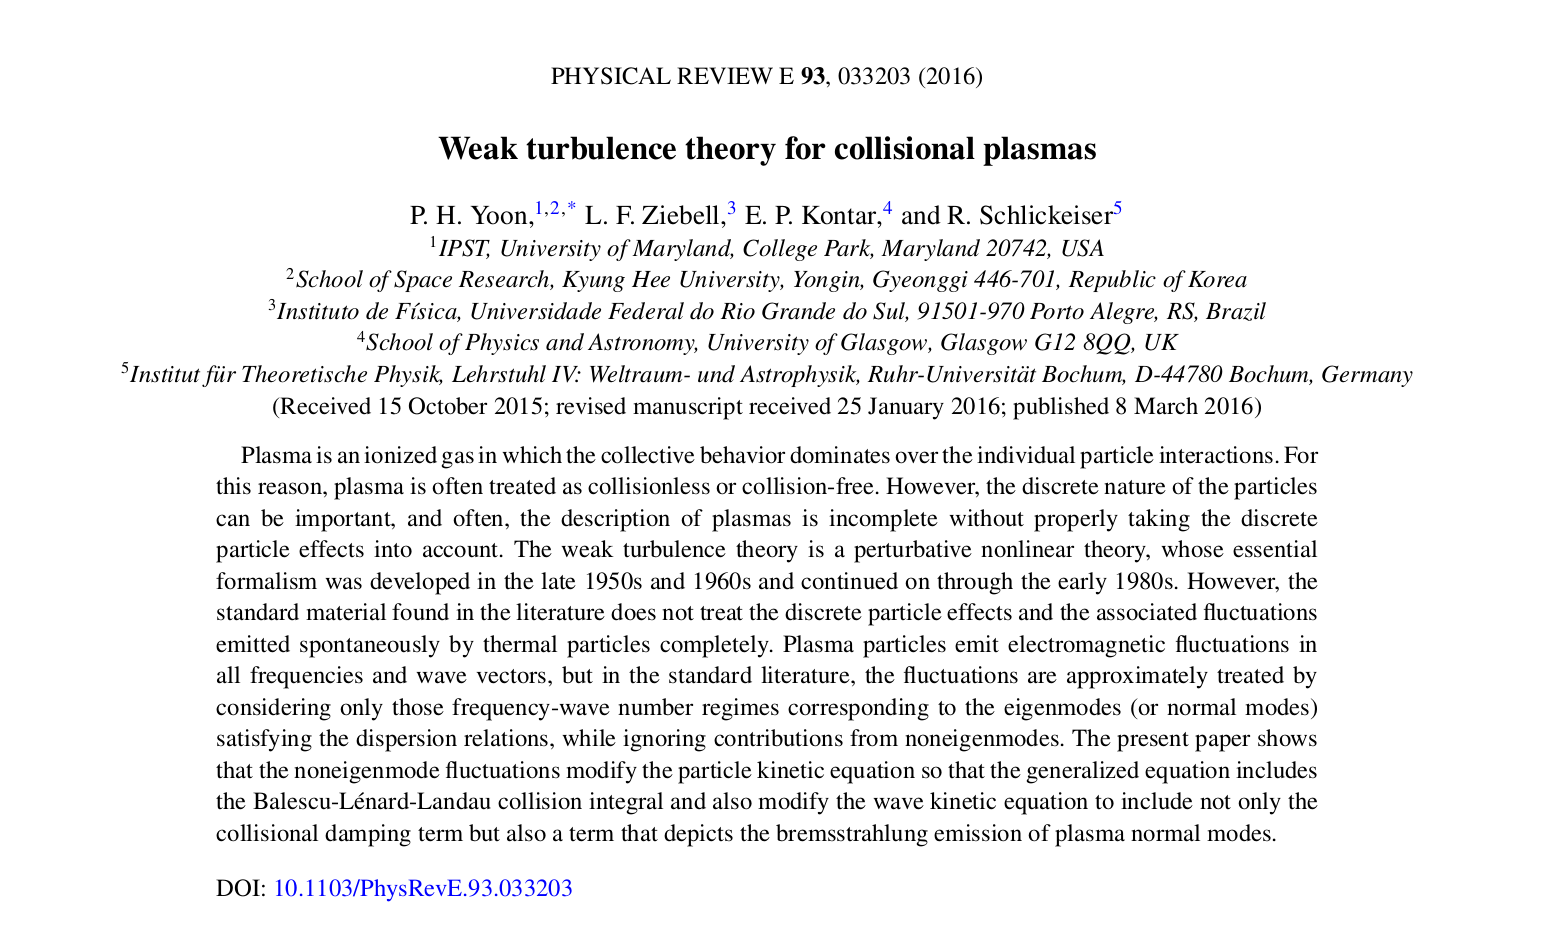
\includegraphics[width=9cm]{print_Yoon2016a.png}
%   \caption*{}
% \end{figure}

\begin{frame}
  \frametitle{Definindo os não automodos}
  \begin{itemize}
    \item Vamos considerar apenas a parte linear da equação
    para o balanço espectral \eqref{nlebe}:
    \begin{equation}
      \label{lin}
      \begin{split}
	\frac{1}{2}\frac{\partial\,\mbox{Re}\,
	  \epsilon({\bf k},\omega)}{\partial \omega}
	\frac{\partial \left<\delta E^2\right>_{{\bf k},\omega}}{\partial t}
	+&\,\mbox{Re}\,\epsilon({\bf k},\omega)
	\left< \delta E^2 \right>_{{\bf k},\omega}
	+i\,\mbox{Im}\,\epsilon({\bf k},\omega)
	\left< \delta E^2 \right>_{{\bf k},\omega}\\
	=&\frac{2}{\pi}\frac{1}{k^2\epsilon^{*}({\bf k},\omega)}
	\sum_a e^2_a\, \int d{\bf v}\,
	\delta(\omega-{\bf k \cdot v})f_a({\bf v}),
      \end{split}
    \end{equation}
    onde $\epsilon({\bf k},\omega)$ é a constante dielétrica:
    \begin{equation}
      \label{dielec}
      \epsilon({\bf k},\omega)=\sum_a \frac{4\pi e^2_a}{m_ak^2}\int d{\bf v}\,
      \frac{{\bf k \cdot}\partial f_a/\partial{\bf v}}{\omega-{\bf k \cdot v}+i0}.
    \end{equation}
    \pause
    \item Tomando a parte real de \eqref{lin}, obtemos
    \begin{equation}
      \label{real}
      \mbox{Re}\, \epsilon({\bf k},\omega)\left[
      \left\langle \delta E^2 \right\rangle_{{\bf k},\omega}
      -\frac{2}{\pi}\frac{1}{k^2|\epsilon({\bf k},\omega)|^2}
      \sum_a e_a^2 \int d{\bf v}\, \delta(\omega-{\bf k \cdot v})
      f_a({\bf v})\right]=0.
    \end{equation}
  \end{itemize}
\end{frame}

\begin{frame}
  \frametitle{Definindo os não automodos}
  \begin{itemize}
    \item Em \eqref{real}, temos duas possibilidades para o
    espaço de número de onda e frequência;
    \vspace{0.15cm}
    \pause
    \item Para a região de $({\bf k},\omega)$ em que
    $|\epsilon({\bf k},\omega)|^2\ne 0$ temos a contribuição
    dos não automodos
    \begin{equation}
      \label{balance}
      \left\langle \delta E^2 \right\rangle_{{\bf k},\omega}
      =\left\langle \delta E^2 \right\rangle_{{\bf k},\omega}^0,
    \end{equation}
    onde
    \begin{equation}
      \label{field-fluc}
      \left\langle \delta E^2 \right\rangle_{{\bf k},\omega}^0
      \equiv \frac{2}{\pi}\frac{1}{k^2|\epsilon({\bf k},\omega)|^2}
      \sum_a e_a^2 \int d{\bf v}\, \delta(\omega-{\bf k \cdot v})
      f_a({\bf v}),
    \end{equation}
    cuja solução está definida apenas para
    $|\epsilon({\bf k},\omega)|^2\ne 0$;
    \vspace{0.15cm}
    \pause
    \item Para os automodos, a solução é dada por
    $\omega = \omega_{\bf k}^\alpha$, o que leva a
    $\epsilon({\bf k},\omega_{\bf k}^\alpha)=0$;
    \vspace{0.15cm}
    \pause
    \item Logo, o denominador será não nulo apenas quando
    $\omega \ne \omega_{\bf k}^\alpha$;
    \vspace{0.15cm}
    \pause
    \item Nesse caso, $\omega$ não satisfaz a relação de dispersão;
    \vspace{0.15cm}
    \pause
    \item Portanto, $\left< \delta E^2 \right>_{{\bf k},\omega}^0$
    representa a contribuição dos modos não normais de oscilação.
  \end{itemize}
\end{frame}

\begin{frame}
  \frametitle{Duas situações distintas}
  \begin{itemize}
    \item Portanto, temos duas situações distintas:
    \vspace{0.1cm}
    \pause
    \begin{itemize}
      \item O formalismo padrão da teoria de turbulência fraca, em que
      apenas os modos normais de oscilação são importantes e a densidade
      de energia das flutuações do campo elétrico é dada por
      \begin{equation*}
	\label{collective}
	\begin{split}
	  \left< \delta E^2 \right>_{{\bf k},\omega}
	  -\left< \delta E^2 \right>_{{\bf k},\omega}^0
	  &=\sum_{\sigma=\pm 1}\sum_{\alpha=L,S}
	  I_{\bf k}^{\sigma \alpha}
	  \delta(\omega-\sigma \omega_{\bf k}^\alpha)\\
	  \mbox{Re}\, \epsilon({\bf k},\sigma\omega_{\bf k}^\alpha)&=0;
	\end{split}
      \end{equation*}
      \vspace{-0.25cm}
      \pause
      \item E o caso em que a densidade de energia espectral pode ser
      descrita da forma apresentada no slide anterior.
    \end{itemize}
    \vspace{0.1cm}
    \pause
    \item Com os automodos, descrevemos os processos coletivos, que
    envolvem ondas e instabilidades cinéticas;
    \vspace{0.1cm}
    \pause
    \item Já a inclusão dos modos não normais, leva a uma nova teoria
    de primeiros princípios que descreve as interações colisionais do
    plasma.
  \end{itemize}
\end{frame}

\begin{frame}
  \frametitle{Generalização da densidade de energia espectral}
  \begin{itemize}
    \item Para incluir as contribuições dos automodos e dos não
    automodos, vamos definir a seguinte quantidade
    \begin{displaymath}
      \Psi_{{\bf k},\omega}\equiv\left< \delta E^2 \right>_{{\bf k},\omega}
      -\left< \delta E^2 \right>_{{\bf k},\omega}^0;
    \end{displaymath}
    \vspace{-0.4cm}
    \pause
    \item A quantidade $\Psi_{{\bf k},\omega}$ representa a
    \emph{autofunção} total que % aparece na equação \eqref{real}
    % \begin{displaymath}
    %   \mbox{Re}\, \epsilon({\bf k},\omega)\Psi_{{\bf k}, \omega}=0;
    % \end{displaymath}\vspace{-0.75cm}
    % \pause
    % \item Onde $\Psi_{{\bf k},\omega}$
    pode ser expressa como
    \begin{displaymath}
      \Psi_{{\bf k},\omega}=\sum_{\sigma=\pm 1}\sum_{\alpha=L,S}
      I_{\bf k}^{\sigma \alpha}\delta(\omega-\sigma \omega_{\bf k}^\alpha),
    \end{displaymath}
    sendo $\sigma \omega_{\bf k}^\alpha$ o autovalor que satisfaz
    $\mbox{Re}\, \epsilon({\bf k},\sigma\omega_{\bf k}^\alpha)=0$;
    \vspace{0.25cm}
    \pause
    \item Com isso, obtemos uma expressão generalizada para as
    flutuações do campo elétrico:
    \begin{equation}
      \label{gen-dens}
      \left< \delta E^2 \right>_{{\bf k},\omega}
      =\left< \delta E^2 \right>_{{\bf k},\omega}^0
      +\sum_{\sigma=\pm 1}\sum_{\alpha=L,S}
      I_{\bf k}^{\sigma \alpha}
      \delta(\omega-\sigma \omega_{\bf k}^\alpha).
    \end{equation} 
  \end{itemize}
\end{frame}

\subsection{Não automodos não alteram a equação quaselinear das  ondas}
\begin{frame}
  \frametitle{Não automodos não alteram a equação
    quaselinear das  ondas}
  \begin{itemize}
    \item Substituindo a equação \eqref{gen-dens} na parte
    imaginária da equação \eqref{lin}, obtemos
    \begin{equation*}
      \begin{split}
	&\frac{\partial\, \mbox{Re}\,
	  \epsilon({\bf k},\omega)}{\partial \omega}
	\frac{\partial \left< \delta E^2
	  \right>_{{\bf k},\omega}^0}{\partial t}
	+2\,\mbox{Im}\,\epsilon({\bf k},\omega)
	\left< \delta E^2\right>_{{\bf k},\omega}^0\\
	&+\sum_{\sigma=\pm 1}\sum_\alpha\biggl[
	\frac{\partial \mbox{Re}\,
	  \epsilon({\bf k},\sigma\omega_{\bf k}^\alpha)}
	{\partial(\sigma\omega_{\bf k}^\alpha)}
	\frac{\partial I_{\bf k}^{\sigma \alpha}}{\partial t}
	+2\,\mbox{Im}\,\epsilon({\bf k},\sigma\omega_{\bf k}^\alpha)
	I_{\bf k}^{\sigma \alpha}\biggr]
	\delta(\omega-\sigma\omega_{\bf k}^\alpha)\\
	&=\mbox{Im}\,\frac{4}{\pi k^2\epsilon^{*}({\bf k},\omega)}
	\sum_a e^2_a\, \int d{\bf v}\,
	\delta(\omega-{\bf k \cdot v})f_a({\bf v});
      \end{split}
    \end{equation*}
    \vspace{-0.4cm}
    \pause
    \item Fazendo uso das propriedades
    \begin{equation*}
      \begin{split}
	\frac{1}{\epsilon({\bf k},\omega)}
	&=\mathcal{P}\frac{1}{\epsilon({\bf k},\omega)}
	-\sum_{\sigma=\pm 1}\sum_{\alpha=L,S}
	\frac{i\pi \delta(\omega-\sigma\omega_{\bf k}^\alpha)}
	{\epsilon '({\bf k},\omega)}\\
	\frac{1}{\epsilon^*({\bf k},\omega)}
	&=\mathcal{P}\frac{1}{\epsilon^*({\bf k},\omega)}
	+\sum_{\sigma=\pm 1}\sum_{\alpha=L,S}
	\frac{i\pi \delta(\omega-\sigma\omega_{\bf k}^\alpha)}
	{\epsilon '({\bf k},\omega)},
      \end{split}
    \end{equation*}
    onde\,
    $ \epsilon '({\bf k},\omega)=\partial\, \mbox{Re}\,
    \epsilon({\bf k},\omega)/\partial \omega$, obtemos\dots
  \end{itemize}
\end{frame}

\begin{frame}
  \begin{itemize}
    \item \dots a seguinte expressão
    \begin{equation*}
      \label{noneigenmode-ql}
      \begin{split}
	\epsilon '({\bf k},\omega)
	&\frac{\partial \left< \delta E^2
	  \right>_{{\bf k},\omega}^0}{\partial t}
	+\mbox{Im}\,\frac{4}{\pi k^2\epsilon^*({\bf k},\omega)}
	\sum_ae_a^2 \int d{\bf v}\,
	\delta(\omega-{\bf k \cdot v})f_a({\bf v})\\
	&+\sum_{\sigma=\pm 1}\sum_\alpha\left[
	  \epsilon '({\bf k},\sigma\omega_{\bf k}^\alpha)
	  \frac{\partial I_{\bf k}^{\sigma \alpha}}{\partial t}
	  +2\,\mbox{Im}\,\epsilon({\bf k},\sigma\omega_{\bf k}^\alpha)
	  I_{\bf k}^{\sigma \alpha}\right]
	\delta(\omega-\sigma\omega_{\bf k}^\alpha)\\
	&=\mbox{Im}\,\mathcal{P}
	\frac{4}{\pi k^2\epsilon^{*}({\bf k},\omega)}
	\sum_a e^2_a\, \int d{\bf v}\,
	\delta(\omega-{\bf k \cdot v})f_a({\bf v})\\
	& +\sum_{\sigma=\pm 1}\sum_\alpha
	\frac{4\delta(\omega-{\bf k \cdot v})}
	{k^2\epsilon '({\bf k},\sigma\omega_{\bf k}^\alpha)}
	\sum_a e^2_a\, \int d{\bf v}\,
	\delta(\omega-{\bf k \cdot v})f_a({\bf v});
      \end{split}
    \end{equation*}
    \pause
    \item De acordo com a definição de
    $\left< \delta E^2\right>_{{\bf k},\omega}^0$,
    o argumento da constante dielétrica exclui os automodos;
    \vspace{0.15cm}
    \pause
    \item Portanto, o segundo termo do lado esquerdo da igualdade é tomado
    com o valor principal, cancelando o primeiro termo do lado direito.
  \end{itemize}
\end{frame}

\begin{frame}
  \frametitle{Equação quaselinear das ondas e os modos não normais de
    oscilação}
  \begin{itemize}
    \item Supondo
    $\partial \left< \delta E^2 \right>_{{\bf k},\omega}^0/\partial
    t=0$ e rearranjando a equação anterior, ficamos com
    \begin{equation*}
      \begin{split}
	\label{eigenmode-ql2}
	\frac{\partial I_{\bf k}^{\sigma \alpha}}{\partial t}
	=-\frac{2\,\mbox{Im}\,\epsilon({\bf k},
	  \sigma\omega_{\bf k}^\alpha)}
	{\epsilon '({\bf k},\sigma\omega_{\bf k}^\alpha)}
	I_{\bf k}^{\sigma \alpha}
	+\frac{4}{k^2[\epsilon '({\bf k},
	  \sigma\omega_{\bf k}^\alpha)]^2} \sum_a e^2_a\,
	\int d{\bf v}\,\delta(\omega-{\bf k \cdot v})f_a({\bf v}),
      \end{split}
    \end{equation*}
    que é a equação cinética quaselinear, com o termo de emissão
    espontânea adicionado;
    \vspace{0.5cm}
    \pause
    \item Logo, podemos concluir que a inclusão dos não automodos
    não altera a equação cinética das ondas na aproximação quaselinear.
  \end{itemize}
\end{frame}


\subsection{Contribuição dos não automodos para a equação
  cinética das partículas}
\begin{frame}
  \frametitle{Contribuição dos não automodos para a equação
    cinética
    das partículas}
  \begin{itemize}
    \item Relembrando a equação cinética generalizada, quaselinear,
    para as partículas:
    \begin{equation*}
      \begin{split}
	\frac{\partial f_a}{\partial t} &=\frac{\pi e_a^2}{m_a^2}
        \int d{\bf k}\,\int d\omega\, \left( \frac{\bf k}{k}\cdot
	\frac{\partial}{\partial {\bf v}}\right)
	\delta(\omega -{\bf k \cdot v})\\
	&\times\left[\mbox{Im} \frac{m_a \epsilon({\bf k},\omega)}
	  {2\pi^3k \left|\epsilon ({\bf k},\omega) \right|^2 } f_a
	  +\left<\delta E^2\right>_{{\bf k},\omega}\left(
            \frac{\bf k}{k} \frac{\partial f_a}{\partial \bf v}
          \right)\right];
      \end{split}
    \end{equation*}\pause
    \item Substituindo $\left< \delta E^2 \right>_{{\bf k},\omega}$
    pela expressão generalizada para a inclusão dos não automodos,
    ficamos com
    \begin{equation*}
      \begin{split}
        \frac{\partial f_a}{\partial t}
	&=\frac{\pi e_a^2}{m_a^2} \int d{\bf k}\, \int d\omega\,
	\left( \frac{\bf k}{k}\cdot \frac{\partial}{\partial {\bf v}}
	\right) \delta(\omega-{\bf k \cdot v}) \biggl[\mbox{Im}\,
	\mathcal{P} \frac{m_a}{2\pi^3k\, \epsilon^*({\bf k},\omega)}
	f_a({\bf v})\\
	&+\frac{2}{\pi k^2|\epsilon({\bf k},\omega)|^2} \sum_b
	e_b^2\int d{\bf v'} \delta(\omega-{\bf k\cdot v'})
	f_b({\bf v '})\left( \frac{\bf k}{k}\cdot
	  \frac{\partial f_a({\bf v})}{\partial {\bf v}}\right)\\
	&+\sum_\sigma\sum_\alpha
	\frac{\pi m_a\,\delta(\omega-\sigma\omega_{\bf k}^\alpha)}
	{2\pi^3 k\, \epsilon '({\bf k},\sigma\omega_{\bf k}^\alpha)}
	f_a({\bf v}) +\sum_\sigma\sum_\alpha I_{\bf k}^{\sigma \alpha}\,
	\delta(\omega-\sigma\omega_{\bf k}^\alpha)
	\left(\frac{\bf k}{k}\cdot
       \frac{\partial f_a({\bf v})}{\partial {\bf v}}\right)\biggr].
      \end{split}
    \end{equation*}
  \end{itemize}
\end{frame}

\begin{frame}
  \frametitle{Então\dots}
  \begin{itemize}
    \item Integrando em $\omega$
    \begin{equation*}
      \begin{split}
	\frac{\partial f_a}{\partial t}
	&=\frac{\pi e_a^2}{m_a^2} \int d{\bf k}\,
	\left( \frac{\bf k}{k}\cdot \frac{\partial}{\partial {\bf v}}
	\right) \biggl[\mathcal{P}
	\frac{m_a\mbox{Im}\,\epsilon({\bf k},{\bf k \cdot v})}
          {2\pi^3k\, |\epsilon({\bf k},{\bf k \cdot v})|^2}f_a({\bf v})\\
	&+\frac{2}{\pi k^2|\epsilon({\bf k},{\bf k \cdot v})|^2} \sum_b
	e_b^2\int d{\bf v'} \delta({\bf k \cdot v}-{\bf k\cdot v'})
	f_b({\bf v '})\left( \frac{\bf k}{k}\cdot
	  \frac{\partial f_a({\bf v})}{\partial {\bf v}}\right)\biggr]\\
	&+\frac{\pi e_a^2}{m_a}\sum_\sigma\sum_\alpha\,
	\int d{\bf k} \left( \frac{\bf k}{k} \cdot
	  \frac{\partial}{\bf v} \right)\,
	\delta(\sigma\omega_{\bf k}^\alpha-{\bf k \cdot v})\\
	&\times\left[ \frac{\pi m_a}{2\pi^3 k\,
	  \epsilon '({\bf k},\sigma\omega_{\bf k}^\alpha)}
	f_a({\bf v}) + I_{\bf k}^{\sigma \alpha}\,
	\left(\frac{\bf k}{k}\cdot
	  \frac{\partial f_a({\bf v})}{\partial {\bf v}}\right) \right]
      \end{split}
    \end{equation*}
    e, fazendo uso da definição de $\mbox{Im}\,\epsilon({\bf k},\omega)$:
    \begin{displaymath}
      \mbox{Im}\epsilon({\bf k},\omega)
      =-\pi \sum_\alpha \frac{4\hat n \pi e_a^2}{m_a k^2}
      \int d{\bf v}\,{\bf k \cdot}
      \frac{\partial F_a}{\partial {\bf v}}
      \delta(\omega-{\bf k\cdot v}),
    \end{displaymath}
    obtemos a equação cinética generalizada para as partículas.
  \end{itemize}
\end{frame}

\begin{frame}
  \frametitle{Equação de Balescu-Lenard}
  \begin{itemize}
    \item Tal equação tem a seguinte forma
    \begin{equation}
      \begin{split}
	\frac{\partial F_a({\bf v})}{\partial t}
	&=\sum_b\frac{2e_a^2e_b^2n_b}{m_a}
	\frac{\partial }{\partial v_i}
	\int d{\bf k}\ \int d{\bf v'}\frac{k_ik_j}{k^4}
	\frac{\delta({\bf k \cdot v - k \cdot v'})}
	{|\epsilon({\bf k, k\cdot v})|^2}\\
	&\times \left(\frac{\partial }{\partial v_j}
	  -\frac{m_a}{m_b}\frac{\partial }{\partial v'_j}
	\right)F_a({\bf v})F_b({\bf v'})\\
	&+\frac{\pi e_a^2}{m_a^2}\sum_\sigma\sum_{\alpha=L,S}
	\int d{\bf k} \biggl(\frac{\bf k}{k}
	\cdot\frac{\partial}{\partial{\bf v}}\biggr)
	\delta(\sigma\omega_{\bf k}^\alpha-{\bf k}\cdot{\bf v})\\
	&\times\biggl(\frac{m_a}{2\pi^2k
	  \epsilon '({\bf k},\sigma\omega_{\bf k}^L)} F_a({\bf v})
	+I_{\bf k}^{\sigma\alpha} \frac{\bf k}{k}\cdot
	\frac{\partial F_a({\bf v})}{\partial{\bf v}}\biggr),
      \end{split}
   \label{Fa-gen}
    \end{equation}
    onde $f_a({\bf v})= \hat n F_a({\bf v}), \quad \int d^3v\ F_a({\bf v})=1$;
    \vspace{0.3cm}
    \item E é composta pela integral colisional de Balescu-Lenard,
    e pelos termos de fricção e de difusão no espaço de velocidades.
  \end{itemize}
\end{frame}

\begin{frame}
  \frametitle{Aproximação}
  \begin{itemize}
    \item A contribuição dos não automodos é mais importante na região
    de maior concentração de partículas, ou seja,  em torno de $v=0$;
    \vspace{0.2cm}
    \item Dessa forma, podemos tratar o argumento de frequência angular
    que aparece na função resposta linear como ${\bf k \cdot v}\approx 0$,
    resultando em
    \begin{displaymath}
      \epsilon({\bf k},{\bf k \cdot v})\approx
      \epsilon({\bf k},0)=1+\sum_a \frac{2 \omega_{pa}^2}{k^2v_{T_a}^2}
      =1+\frac{2 \omega_{pe}^2}{k^2v_{Te}^2}\left( 1+\frac{T_e}{T_i} \right)
    \end{displaymath}\vspace{-0.4cm}
    \pause
    \item O que leva à seguinte expressão
  \end{itemize}
  \vspace{0.3cm}
  \begin{equation*}
    \hspace{-0.85cm}
    \begin{split}
      \frac{\partial F_a({\bf v})}{\partial t}
      &=\sum_b\frac{2e_a^2e_b^2n_b}{m_a}
      \frac{\partial }{\partial v_i}\int d{\bf k}\ \int d{\bf v'}\,
      \frac{k_ik_j\lambda_{De}^4 \delta({\bf k \cdot v - k \cdot v'})}
      {|1+T_e/T_i+k^2 \lambda_{De}^2|^2} \left(\frac{\partial }{\partial v_j}
	-\frac{m_a}{m_b}\frac{\partial }{\partial v'_j}\right)
      F_a({\bf v})F_b({\bf v'})\\
      &+\frac{\pi e_a^2}{m_a^2}\sum_\sigma\sum_{\alpha=L,S}
      \int d{\bf k} \biggl(\frac{\bf k}{k}
      \cdot\frac{\partial}{\partial{\bf v}}\biggr)
      \delta(\sigma\omega_{\bf k}^\alpha-{\bf k}\cdot{\bf v})
      \biggl(\frac{m_a}{2\pi^2k\epsilon '({\bf k},\sigma\omega_{\bf k}^L)}
      F_a({\bf v})+I_{\bf k}^{\sigma\alpha} \frac{\bf k}{k}\cdot
      \frac{\partial F_a({\bf v})}{\partial{\bf v}}\biggr).
    \end{split}
  \end{equation*}  
\end{frame}

\subsection{Contribuição dos não automodos para a equação cinética  não linear das ondas}
\begin{frame}
  \frametitle{Contribuição dos não automodos para a equação cinética
    não linear das ondas}
  \begin{itemize}
    \item Considerando os termos não lineares da equação para o balanço
    espectral \eqref{nlebe};
    \vspace{0.4cm}
    \pause
    \item Vamos desconsiderar todas as flutuações dos não automodos
    com argumento ${\bf k}$ e $\omega$, uma vez que os não automodos
    não estão definidas na região em que $\omega=\sigma \omega_{\bf k}$;
    \vspace{0.4cm}
    \pause
    \item As flutuações com outros argumentos, no entanto, devem ser
    mantidas;
    \vspace{0.4cm}
    \pause
    \item Não queremos descrever os não automodos em si, e
    sim a influência deles sobre as emissões no intervalo de
    frequência dos modos normais de oscilação do plasma;
    \vspace{0.4cm}
    \pause
    \item Com isso, obtemos a forma generalizada da equação para o
    balanço espectral:    
  \end{itemize}
\end{frame}

\begin{frame}
  \vspace{-0.6cm}
  \begin{displaymath}
    \begin{split}
      \mbox{NL}
      =&-2\int d{\bf k'} \int d\omega '\,\biggl\{
      \left[\chi^{(2)}({\bf k'},\omega '|{\bf k - k'},
	\omega-\omega ')\right]^2\\
      &\times\biggl[\frac{\left< \delta E^2 \right>_{{\bf k-k'},\omega-\omega '}^0
	+\sum_{\sigma ''}\sum_{\gamma} I_{\bf k -k'}^{\sigma '' \gamma}
	\delta(\omega-\omega ' -\sigma '' \omega_{\bf k -k'}^\gamma)}
      {\epsilon({\bf k'},\omega ')}\\
      &+\frac{\left< \delta E^2 \right>_{{\bf k'},\omega '}^0
	+\sum_{\sigma '}\sum_{\beta}
	I_{\bf k'}^{\sigma ' \beta}\delta(\omega '-\sigma ' \omega_{\bf k'}^\beta)}
      {\epsilon({\bf k-k'},\omega-\omega ')}\biggr]
      -\bar \chi^{(3)}({\bf k'},\omega|-{\bf k'},-\omega '|{\bf k},\omega)\\
      &\times\biggl[ \left< \delta E^2 \right>_{{\bf k'},\omega '}^0
      +\sum_{\sigma '}\sum_{\beta}I_{\bf k'}^{\sigma ' \beta}
      \delta(\omega '-\sigma ' \omega_{\bf k'}^\beta) \biggr]\biggr\}
      \sum_{\sigma}\sum_{\alpha}
      I_{\bf k}^{\sigma \alpha}\delta(\omega-\sigma \omega_{\bf k}^\alpha)\\
      &+2\int d{\bf k'} \int d\omega '
      \frac{|\chi^{(2)}({\bf k'},\omega '|{\bf k-k'},\omega-\omega ')|^2}
      {\epsilon^*({\bf k},\omega)}\biggl[
      \left< \delta E^2 \right>_{{\bf k'},\omega '}^0
      +\sum_{\sigma '}\sum_{\beta}I_{\bf k'}^{\sigma ' \beta}
      \delta(\omega '-\sigma ' \omega_{\bf k'}^\beta) \biggr]\\
      &\times \biggl[ \left< \delta E^2 \right>_{{\bf k - k'},\omega-\omega '}^0
      +\sum_{\sigma ''}\sum_{\gamma} I_{\bf k -k'}^{\sigma '' \gamma}
      \delta(\omega-\omega ' -\sigma '' \omega_{\bf k -k'}^\gamma) \biggr]
    \end{split}
  \end{displaymath}
\end{frame}

\begin{frame}[noframenumbering]
  \begin{displaymath}
    \begin{split}
      &-\frac{4}{\pi}\int d{\bf k '} \int d\omega '\,
      \frac{1}{k^2|\epsilon({\bf k'},\omega ')|^2}\biggl\{
      \frac{[\chi^{(2)}({\bf k'},\omega '|{\bf k-k'},\omega
	-\omega ')]^2}{\epsilon({\bf k - k'},\omega-\omega ')}
      \sum_{\sigma}\sum_{\alpha}I_{\bf k}^{\sigma \alpha}
      \delta(\omega-\sigma \omega_{\bf k}^\alpha)\\
      &-\frac{|\chi^{(2)}({\bf k'},\omega '|{\bf k-k'},\omega-\omega ')|^2}
      {\epsilon^*({\bf k},\omega)}\biggl[
      \left< \delta E^2 \right>_{{\bf k - k'},\omega-\omega '}^0
      +\sum_{\sigma ''}\sum_{\gamma}I_{\bf k -k'}^{\sigma '' \gamma}
      \delta(\omega-\omega ' -\sigma '' \omega_{\bf k -k'}^\gamma)
      \biggr]\biggr\}\\
      &\times\sum_ae_a^2\int d{\bf v}\,
      \delta(\omega '-{\bf k \cdot v})F_a({\bf v})\\
      -&\frac{4}{\pi}\int d{\bf k '} \int d\omega '\
      \frac{1}{|{\bf k - k'}|^2|\epsilon({\bf k-k'},\omega-\omega ')^2}
      \biggl\{ \frac{[\chi^{(2)}({\bf k'},\omega '|{\bf k-k'},\omega
	-\omega ')]^2}{\epsilon({\bf k'},\omega ')}\\
      &\times\sum_{\sigma}\sum_{\alpha} I_{\bf k}^{\sigma \alpha}
      \delta(\omega-\sigma \omega_{\bf k}^\alpha)
      -\frac{|\chi^{(2)}({\bf k'},\omega '|{\bf k-k'},\omega-\omega ')|^2}
      {\epsilon^*({\bf k},\omega)}\\
      &\times \biggl[\left< \delta E^2 \right>_{{\bf k'},\omega '}^0
      +\sum_{\sigma '}\sum_{\beta}I_{\bf k'}^{\sigma ' \beta}
      \delta(\omega '-\sigma ' \omega_{\bf k'}^\beta)\biggr]\biggr\}
      \sum_a e_a^2\int d{\bf v}\,
      \delta(\omega-\omega '-{\bf (k-k')\cdot v})F_a({\bf v}).
    \end{split}
  \end{displaymath}
\end{frame}

\begin{frame}
  \frametitle{Termos de correção dos não automodos para a equação
    cinética das ondas}
  \begin{itemize}
    \item Integrando em $\omega '$ e decompondo os denominadores
    $1/\epsilon({\bf k-k'},\sigma \omega_{\bf k}^\alpha-{\bf k'\cdot v})$
    e $1/\epsilon^*({\bf k},\omega)$, como feito para a equação quaselinear,
    obtemos os termos de correção: %\vspace{-0.25cm}
    \begin{equation*}
      \label{corr}
      \begin{split}
	\mbox{corr}&=-\sum_{\sigma '}\sum_\beta\sum_a \,8\pi e_a^2
	\int d{\bf k'}\int d{\bf v}\,
	\frac{|\chi^{(2)}({\bf k'},\sigma '\omega_{\bf k'}^\beta
	  |{\bf k-k'},({\bf k-k'}){\bf \cdot v})|^2}
	{|{\bf k-k'}|^2|\epsilon[{\bf k-k'},{\bf k-k'},
	  ({\bf k-k'}){\bf \cdot v}]|^2}\\
	&\times \left[ \frac{I_{\bf k}^{\sigma \alpha}}
	  {\epsilon '({\bf k'},\sigma '\omega_{\bf k'}^\beta)}
	  -\frac{I_{\bf k'}^{\sigma '\beta}}
	  {\epsilon '({\bf k},\sigma \omega_{\bf k}^\alpha)}\right]
	\delta[\sigma\omega_{\bf k}^\alpha-\sigma '\omega_{\bf k'}^\beta
	-({\bf k-k'}){\bf \cdot v}]f_a({\bf v})\\
	&-\sum_a \frac{4 e_a^2}{\pi}
	\int d{\bf k '}\int d{\bf v}\,\mbox{Im}\biggl[ \mathcal{P}\,
	\frac{2[\chi^{(2)}({\bf k'},{\bf k' \cdot v}|{\bf k-k'},
	  \sigma\omega_{\bf k}^\alpha-{\bf k'\cdot v})]^2}
	{\epsilon({\bf k-k'},\sigma \omega_{\bf k}^\alpha
	  -{\bf k'\cdot v})}\\
	&-\bar \chi^{(3)}({\bf k'},{\bf k' \cdot v}|{\bf -k'},
	{\bf -k'\cdot v}|{\bf k},\sigma\omega_{\bf k}^\alpha)\biggr]
	\frac{I_{\bf k}^{\sigma \alpha}}{k'^2|\epsilon({\bf k'},
	  {\bf k'\cdot v})|^2}f_a({\bf v})\\
	&+\sum_a\sum_b \frac{24 e_a^2 e_b^2}{\pi}\int d{\bf k '}
	\int d{\bf v} \int d{\bf v'}\,
	\frac{|\chi^{(2)} \left[ {\bf k'},{\bf k' \cdot v'}|
	    {\bf k-k'},({\bf k-k'}){\bf \cdot v} \right]|^2}
	{k'^2|{\bf k-k'}|^2|\epsilon({\bf k'},{\bf k'\cdot v'})|^2
	  |\epsilon({\bf k-k'},({\bf k-k'}){\bf \cdot v})|^2}\\
	&\times \frac{\delta \left[ \sigma\omega_{\bf k}^\alpha
	    -{\bf k \cdot v}+{\bf k' \cdot}({\bf v-v'})\right]}
	{\epsilon '({\bf k},\sigma\omega_{\bf k}^\alpha)}
	f_a({\bf v}) f_b({\bf v'}).
      \end{split}
    \end{equation*}
  \end{itemize}
\end{frame}

\begin{frame}
  \frametitle{Aproximação para as funções resposta}
  \begin{itemize}
    % \item Para aproximar as diversas funções resposta em que
    % ${\bf k\cdot v}$ aparece no lugar de $\omega$, precisamos
    % lembrar que ondas não são submetidas a blindagem de Debye;
    % \vspace{0.4cm}
    % \pause
    % \item O que significa que não podemos aplicar a aproximação
    % de acoplamento fraco, que assume $k^2\lambda_{De}^2\gg 1$,
    % levando a $\epsilon({\bf k},0) \approx 1$ e à integral
    % colisional de Landau;
    % \vspace{0.4cm}
    % \pause
    \item Para aproximar as diversas funções resposta em que
    ${\bf k\cdot v}$ aparece no lugar de $\omega$, vamos usar
    a mesma aproximação aplicada à  equação de Balescu-Lenard:
    \begin{equation*}
      \epsilon({\bf k},{\bf k \cdot v})
      = 1+\left( 2 \frac{\omega_{pe}^2}{k^2v_{Te}^2} \right)
      \left( 1+\frac{T_e}{T_i} \right);
    \end{equation*}
%    \vspace{0.5cm}
    \pause
    \item Com isso obtemos a equação cinética generalizada das
    ondas, que inclui a contribuição dos modos não normais de
    oscilação.
  \end{itemize}
\end{frame}

\begin{frame}
  \frametitle{Equação cinética generalizada das ondas}
  \begin{eqnarray}
  \frac{\partial I^\alpha_{\bf k}}{\partial t}
    &=&-\frac{2 \mbox{Im}\ \epsilon({\bf k}, \sigma \omega_{\bf k}^\alpha)}
    {\epsilon '({\bf k},\sigma \omega_{\bf k}^\alpha)}I^\alpha_{\bf k}
    +\sum_a\frac{4e^2}{k^2[\epsilon '({\bf k},\sigma\omega_{\bf k}^\alpha)]^2}
    \int d{\bf v}\, \delta(\sigma\omega_{\bf k}^\alpha-{\bf k \cdot v})f_a({\bf v})
	\nonumber\\
      &&-4\pi \sum_{\alpha,\beta,\gamma}\ \sum_{\sigma ',\sigma ''}\int d{\bf k '}\
    \frac{|\chi^{(2)}({\bf k'},\sigma '\omega_{\bf k'}^\beta|{\bf k-k'},
      \sigma ''\omega_{\bf k-k'}^\gamma)|^2}
    {\epsilon '({\bf k},\sigma \omega_{\bf k}^{\alpha})}
    \nonumber\\
      &&\times \biggl(\frac{I_{\bf k-k'}^{\gamma}\ I_{\bf k}^{\alpha}}
       {\epsilon '({\bf k'},\sigma ' \omega_{\bf k'}^{\beta})}
       +\frac{I_{\bf k'}^{\beta}\ I_{\bf k}^{\alpha}}
       {\epsilon '({\bf k-k'},\sigma ''\omega_{\bf k-k'}^{\gamma})}
       -\frac{I_{k'}^{\beta}\ I_{\bf k-k'}^{\gamma}}
       {\epsilon '({\bf k},\sigma \omega_{\bf k}^{\alpha})}\biggr)
       \delta\bigl(\sigma \omega_{\bf k}^{\alpha}-\sigma ' \omega_{\bf k'}^{\beta}
	 -\sigma '' \omega_{\bf k-k'}^{\gamma}\bigr)
    \nonumber\\
    &&-\sum_{\alpha,\beta}\ \sum_{\sigma '}
    \int d{\bf k '}\ A_{\alpha,\beta}({\bf k,k'})
    I_{\bf k'}^{\beta}\ I_{\bf k}^{\alpha}
       -\sum_a\,\frac{16 e_a^2}{\epsilon '({\bf k},\sigma\omega_{\bf k}^\alpha)}
       \sum_{\sigma '}\sum_{\beta}
    \nonumber\\
    &&\times\int d{\bf v}\int d{\bf k '}\,
    \frac{|\chi^{(2)}({\bf k'},\sigma '\omega_{\bf k'}^{\beta}|{\bf k-k'},
      \sigma \omega_{\bf k}^\alpha-\sigma '\omega_{\bf k'}^{\beta})|^2}
    {|{\bf k-k'}|^2|\epsilon({\bf k-k'},\sigma \omega_{\bf k}^\alpha
      -\sigma '\omega_{\bf k'}^{\beta})|^2}
    \nonumber\\
    &&\times \left[ \frac{I_{\bf k}^{\sigma \alpha}}
      {\epsilon({\bf k '},\sigma '\omega_{\bf k'}^\beta)}
    -\frac{I_{\bf k'}^{\sigma '\beta}}
    {\epsilon '({\bf k },\sigma \omega_{\bf k}^\alpha)}\right]
   \delta[\sigma \omega_{\bf k}^\alpha-\sigma '\omega_{\bf k'}^\beta
       -({\bf k-k'}){\bf \cdot v}] f_a({\bf v})
       \nonumber
  \end{eqnarray}
\end{frame}
\begin{frame}[noframenumbering]
  \begin{eqnarray*}
       &&\textcolor{darkblue}{
       -\sum_a \,\frac{16 e_a^2}{\epsilon '({\bf k},\sigma\omega_{\bf k}^\alpha)}
       \sum_{\sigma '}\sum_\beta\,
    \int d{\bf k'}\int d{\bf v}\,
       \frac{|{\bf k-k'}|^2 \lambda_{De}^4
       |\chi^{(2)}({\bf k'},\sigma '\omega_{\bf k'}^\beta|{\bf k-k'},0)|^2}
    {|1+T_e/T_i+|{\bf k-k'}|^2 \lambda_{De}^2|^2}}
    \nonumber\\
    &&\textcolor{darkblue}{\times \left[ \frac{I_{\bf k}^{\sigma \alpha}}
      {\epsilon '({\bf k'},\sigma '\omega_{\bf k'}^\beta)}
      -\frac{I_{\bf k'}^{\sigma '\beta}}
	{\epsilon '({\bf k},\sigma \omega_{\bf k}^\alpha)}\right] 
    \delta[\sigma\omega_{\bf k}^\alpha-\sigma '\omega_{\bf k'}^\beta
    -({\bf k-k'}){\bf \cdot v}]f_a({\bf v})}
	 \nonumber\\
      &&\textcolor{skobeloff}{-\sum_a \frac{8 e_a^2}{\pi}
	 \int d{\bf k '}\int d{\bf v}\,
	 \frac{k'^2\lambda_{De}^4}{|1+T_e/T_i+k'^2\lambda_{De}^2|^2}}
	 \nonumber\\
    &&\textcolor{skobeloff}{
     \times\mbox{Im}\biggl[ \mathcal{P}\,
    \frac{2[\chi^{(2)}({\bf k'},0|{\bf k-k'},\sigma\omega_{\bf k}^\alpha)]^2}
    {\epsilon({\bf k-k'},\sigma \omega_{\bf k}^\alpha)}
       -\bar \chi^{(3)}({\bf k'},0|{\bf -k'},0|{\bf k},\sigma\omega_{\bf k}^\alpha)\biggr]
       I_{\bf k}^{\sigma \alpha}f_a({\bf v})}
      \nonumber\\
 &&\textcolor{softred}{+\sum_a\sum_b
     \frac{48 e_a^2 e_b^2}{\pi[\epsilon '({\bf k},\sigma\omega_{\bf k}^\alpha)]^2}
     \int d{\bf k '} \int d{\bf v} \int d{\bf v'}\,
     \frac{k'^2|\chi^{(2)} \left( {\bf k'},0|{\bf k-k'},0 \right)|^2}
     {|1+T_e/T_i+k^2 \lambda_{De}^2|^2}}
    \nonumber\\
  &&\textcolor{softred}{\times \frac{|{\bf k-k'}|^2\lambda_{De}^8}
     {|1+T_e/T_i+|{\bf k-k'}|^2 \lambda_{De}^2|^2} 
     \delta \left[ \sigma\omega_{\bf k}^\alpha-{\bf k \cdot v}
	+{\bf k' \cdot}({\bf v-v'})\right] f_a({\bf v}) f_b({\bf v'})}.
       \label{wave-gen}
\end{eqnarray*}
\end{frame}

\begin{frame}
  \frametitle{Correção para o espalhamento espontâneo}
  \begin{itemize}
    \item O termo em azul claro é um termo de correção para o efeito
    de emissão espontânea, cuja forma final é a seguinte
  \end{itemize}
    \vspace{0.2cm}
    \begin{equation*}
      \begin{split}
	u_{k,k'}^{L\, (\mbox{\tiny corr})} &=
	-\frac{\hat n e^2}{m_e^2\omega_{pe}^4}\sigma \omega_{\bf k}^L
	\sum_{\sigma '} \int d{\bf k'}\int d{\bf v}\,
	\frac{({\bf k-k'})^2}{k^2 k'^2|1+T_e/T_i+({\bf k-k'})^2\lambda_{De}^2|^2}\\
	&\times \left( \sigma '\omega_{\bf k'}^L I_{\bf k}^{\sigma L}
	  -\sigma \omega_{\bf k}^L I_{\bf k'}^{\sigma 'L}\right)
	\delta[\sigma\omega_{\bf k}^L-\sigma '\omega_{\bf k'}^L
	-({\bf k-k'}){\bf \cdot v}]\left[ F_e({\bf v}) +F_i({\bf v})\right],
      \end{split}
    \end{equation*}
    \vspace{0.3cm}
    \begin{equation*}
      \begin{split}
	u_{k,k'}^{S\, (\mbox{\tiny corr})} &=
	-\frac{\hat n e^2}{m_e^2\omega_{pe}^4}\mu_{\bf k}\mu_{\bf k'}
	\sigma \omega_{\bf k}^L \sum_{\sigma '} \int d{\bf k'}
	\int d{\bf v}\, \frac{1}{k^2 k'^2\lambda_{De}^4}
	\left(1-\frac{T_e}{T_i} \frac{\bf k \cdot k'}{k'^2} \right)^2\\
	&\times	\left[1+\frac{T_e}{T_i}+({\bf k-k'})^2 \lambda_{De}^2
	\right]^{-2}\left( \sigma '\omega_{\bf k'}^S I_{\bf k}^{\sigma S}
	  -\sigma \omega_{\bf k}^S I_{\bf k'}^{\sigma 'S}\right)\\
	&\times \delta[\sigma\omega_{\bf k}^S-\sigma '\omega_{\bf k'}^S
	-({\bf k-k'}){\bf \cdot v}]\left[ F_e({\bf v}) +F_i({\bf v})\right].
      \end{split}
    \end{equation*}
\end{frame}

\begin{frame}
  \frametitle{Espalhamento espontâneo corrigido para ondas $L$ e $S$}
  \begin{itemize}
    \item Substituindo no termo de espalhamento espontâneo, ficamos com as
    seguintes expressões para as ondas $L$ e $S$
  \end{itemize}
  \vspace{0.2cm}
  \begin{equation*}
    \begin{split}
      u_{k,k'}^{L}&=\sigma\omega_{\bf k}^L\,
      \frac{\hat n e^4}{m_e^2\,\omega_{pe}^4}
      \sum_{\sigma '}\int d{\bf k'}\int d{\bf v}\;
      \frac{({\bf k}\cdot{\bf k}')^2}{k^2\,k'^2}\;
      \delta[\sigma\omega_{\bf k}^L-\sigma '\omega_{{\bf k}'}^L
      -({\bf k}-{\bf k}')\cdot{\bf v}]\\
      &\times\,\bigl(\sigma\omega_{\bf k}^L\,I_{{\bf k}'}^{\sigma 'L}
      -\sigma '\omega_{{\bf k}'}^L\, I_{\bf k}^{\sigma L}\bigr)
      \left[1\textcolor{darkblue}{
	  + \frac{1}{|1+T_e/T_i+({\bf k-k'})^2 \lambda_{De}^2|^2}}
      \right] \,[F_e({\bf v})+F_i({\bf v})],
    \end{split}
  \end{equation*}
  \vspace{0.3cm}
  \begin{equation*}
    \begin{split}
      u_{k,k'}^{S}&=\sigma\omega_{\bf k}^L
      \frac{\hat n e^4}{m_e^2\omega_{pe}^4}
      \frac{\mu_{\bf k}}{k^2\lambda_{De}^4}\sum_{\sigma '}
      \int d{\bf k'}\,\frac{\mu_{{\bf k}'}}{k'^2}
      \int d{\bf v}\,[F_e({\bf v})+F_i({\bf v})]\\
      &\times\left(\sigma\omega_{\bf k}^L
	\frac{I_{{\bf k}'}^{\sigma 'S}}{\mu_{{\bf k}'}}
	-\sigma '\omega_{{\bf k}'}^L
	\frac{I_{\bf k}^{\sigma S}}{\mu_{\bf k}}\right)
      \delta[\sigma\omega_{\bf k}^S-\sigma '\omega_{{\bf k}'}^S
      -({\bf k}-{\bf k}')\cdot{\bf v}]\\
      &\times\left[\frac{({\bf k}\cdot{\bf  k}')^2}{k^2k'^2}
	W_{{\bf k},{\bf k}'}\textcolor{darkblue}{
	  +\frac{\left(1-\frac{T_e}{T_i}
	      \frac{\bf k \cdot k'}{k'^2}\right)^2}
	  {|1+T_e/T_i+({\bf k-k'})^2 \lambda_{De}^2|^2}}\right].
    \end{split}
  \end{equation*}
\end{frame}

\begin{frame}
  \frametitle{Amortecimento colisional para ondas $L$ e $S$}
  \begin{itemize}
    \item Tomando as devidas aproximações do termo em verde, obtemos
    as equações para o amortecimento colisional das ondas $L$ e $S$:
    \vspace{0.2cm}
    \begin{equation*}
      \begin{split}
	\gamma_{\bf k}^{\sigma L\,(\mbox{\tiny coll})}
	&= \sigma \omega_{\bf k}^L
	\frac{4\hat{n}e^4\omega_{pe}^2}{T_e^2}\int d{\bf k}'
	\frac{({\bf k}\cdot {\bf k'})^2\lambda_{De}^4}{k^2k'^4|
	  \epsilon({\bf k'},\sigma\omega_{\bf k}^L)|^2}\\
	&\times \left(1+\frac{T_e}{T_i}+({\bf k}-{\bf k'})^2
	  \lambda_{De}^2\right)^{-2}\int d{\bf v}\, {\bf k'}
	\cdot \frac{\partial F_e({\bf v})}{\partial {\bf v}}
	\delta [\sigma\omega_{\bf k}^L-{\bf k'}\cdot{\bf v}]
      \end{split}
    \end{equation*}
    \vspace{0.3cm}
    \begin{equation*}
      \begin{split}
	\gamma_{\bf k}^{\sigma S\, (\mbox{\tiny coll})}
	&= \sigma\mu_{\bf k}\omega_{\bf k}^L
	\frac{\hat{n}e^4\omega_{pe}^2}{T_e^2}\int d{\bf k}'
	\frac{1}{k^2k'^4 |\epsilon({\bf k'},\sigma\omega_{\bf k}^S)|^2}\\
	&\times \left(1+\frac{T_e}{T_i}+({\bf k}-{\bf k'})^2
	  \lambda_{De}^2\right)^{-2}\left(1+\frac{2T_e}{T_i}
	  \frac{{\bf k}\cdot{\bf k}'}{k^2}\right)\\
	&\times \int d{\bf v}\, {\bf k'}
	\cdot\frac{\partial}{\partial{\bf v}}
	\left(F_e({\bf v})+\frac{m_e}{m_i}F_i({\bf v})\right)
	\delta[\sigma\omega_{\bf k}^S-{\bf k'}\cdot{\bf v}].
      \end{split}
    \end{equation*}
  \end{itemize}
\end{frame}

\begin{frame}
    \frametitle{\emph{Bremsstrahlung} eletrostático}
  \begin{itemize}
    \item O termo em rosa, descreve o processo de emissão de
    \emph{bremsstrahlung}  eletrostático, um efeito até então
    desconhecido, cujas equações para ondas $L$ e $S$ são
    as seguintes
    \vspace{0.3cm}
    \begin{equation*}
      \label{PkL,1}
      \begin{split}
	\frac{\partial I_{\bf k}^{\sigma L}}{\partial t}
	\biggr|_{\mbox{\tiny brem}}&=\sum_{a,b}
	\frac{12n_ee_a^2e_b^2\omega_{pe}^2}{\pi}\int d{\bf k}'
	\int d{\bf v}\int d{\bf v}'\,
	\frac{|\chi^{(2)}({\bf k}',0|{\bf k}-{\bf k}',0)|^2}
	{k'^2|{\bf k}-{\bf k}'|^2|\epsilon({\bf k}',0)|^2|
	  \epsilon({\bf k}-{\bf k}',0)|^2}\\
	&\times\delta\left[\sigma\omega_{\bf k}^L-{\bf k}\cdot
	  {\bf v}+{\bf k}'\cdot({\bf v}-{\bf v}')\right]
	F_a({\bf v})F({\bf v}'),\\
      \end{split}
    \end{equation*}
    \vspace{0.4cm}
    \begin{equation*}
      \label{PkS,1}
      \begin{split}
	\frac{\partial}{\partial t}
	\frac{I_{\bf k}^{\sigma S}}{\mu_{\bf k}}\biggr|_{\mbox{\tiny brem}}
	&=\sum_{a,b}\frac{12n_ee_a^2e_b^2\omega_{pe}^2}{\pi}
	\int d{\bf k}'\int d{\bf v}\int d{\bf v}'\,
	\frac{|\chi^{(2)}({\bf k}',0|{\bf k}-{\bf k}',0)|^2}
	{k'^2|{\bf k}-{\bf k}'|^2|\epsilon({\bf k}',0)|^2|
	  \epsilon({\bf k}-{\bf k}',0)|^2}\\
	&\times\delta\left[\sigma\omega_{\bf k}^S-{\bf k}
	  \cdot{\bf v}+{\bf k}'\cdot ({\bf v}-{\bf v}')\right]
	F_a({\bf v})F({\bf v}').
      \end{split}
    \end{equation*}
  \end{itemize}
\end{frame}

\begin{frame}
  \frametitle{Aproximação para a susceptibilidade dielétrica de segunda
    ordem}
  \begin{itemize}
    \item Originalmente, a susceptibilidade dielétrica de segunda
    ordem foi aproximada supondo ${\bf k \cdot v}\approx 0$,
    ${\bf k'\cdot v'}\approx 0$ e ${\bf k' \cdot v}\approx 0$,
    resultando em
    \begin{equation*}
      \chi^{(2)}({\bf k}',0|{\bf k}-{\bf k}',0)
      =-i \sum_a\frac{e_a}{T_a}
      \frac{\omega_{pa}^2}{k k' |{\bf k-k'}|}\frac{1}{v_{Ta}^2}
      =\frac{i e}{T_e}\frac{1}{v_{Te}^2}\left( 1-\frac{T_e^2}{T_i^2}
      \frac{\omega_{pe}^2}{k k' |{\bf k-k'}|}\right),
    \end{equation*}
    que pode ser escrita tanto para ondas $L$ quanto para ondas $S$;
    \pause
    \item Essa aproximação foi revisada para uma forma mais adequada,
    na qual mantemos a condição de ressonância
    ${\bf k'\cdot v'}+({\bf k-k'})\cdot{\bf v}=\sigma\omega_{\bf k}^\alpha$
    no denominador e prosseguimos com a aproximação sob a mesma suposição;
    \pause
    \vspace{0.1cm}
    \item Nesse caso, ficamos com a seguinte expressão 
    \begin{equation*}
      \chi^{(2)}[{\bf k'},{\bf k'\cdot v'}|{\bf k-k'},({\bf k-k'})\cdot{\bf v}]
      \simeq i\frac{2e}{T_e}\frac{\omega_{pe}^2}{k(\omega_{\bf k}^L)^2}
      \left(1-\frac{m_e}{m_i}\frac{T_e}{T_i}\right);
    \end{equation*}
    \pause
    \vspace{-0.3cm}
    \item Tal condição é válida apenas para o modo de oscilação
    predominante que, na dinâmica dos elétrons, são as ondas de
    Langmuir.    
  \end{itemize}
\end{frame}

\begin{frame}
  \frametitle{Bremsstrahlung eletrostático para ondas $(L)$ e $(S)$}
  \begin{itemize}
    \item Para ondas $L$, usando a ``nova'' aproximação, obtemos a seguinte
    expressão para o bremsstrahlung eletrostático
  \end{itemize}
   \vspace{0.1cm}
    \begin{equation*}
    \label{PkL}
    \begin{split}
      P_{\bf k}^{\sigma L} &=
      \frac{3e^2}{4\pi^3}\frac{1}{(\omega_{\bf k}^L)^2}
      \left(1-\frac{m_e}{m_i}\frac{T_e}{T_i}\right)^2\frac{v_e^4}{k^2}
      \int d{\bf k}'k'^2|{\bf k- k'}|^2\left(1+\frac{T_e}{T_i}
	+({\bf k}-{\bf k}')^2\lambda_D^2\right)^{-2}\\
      &\times\left(1+\frac{T_e}{T_i} +{k'}^2\lambda_D^2\right)^{-2}
      \int d{\bf v}\int d{\bf v}'\,
      \delta[\sigma \omega_{\bf k}^L-{\bf k \cdot v}
      +{\bf k'\cdot}({\bf v}-{\bf v '})]
      \sum_aF_a({\bf v})\sum_bF_b({\bf v '})
    \end{split}
  \end{equation*}\pause
  \begin{itemize}
    \item Para ondas $S$, usando a aproximação ``original'', o termo
    de bremsstrahlung eletrostático é dado por
  \end{itemize}
   \vspace{0.1cm}
  \begin{equation*}
    \label{PkS}
    \begin{split}
      P_{\bf k}^{\sigma S} &= \mu_{\bf k}\frac{3e^2T_e}{16\pi^3m_e}
      \biggl(1-\frac{T_e^2}{T_i^2}\biggr)^2\frac{1}{k^2\lambda_D^2}
      \int d{\bf k '}\left(1+\frac{T_e}{T_i}
	+({\bf k}-{\bf k '})^2\lambda_D^2\right)^{-2}\\
      & \times\left(1+\frac{T_e}{T_i}
	+{k'}^2\lambda_D^2\right)^{-2}\int d{\bf v}\int d{\bf v '}\,
      \delta[\sigma\omega_{\bf k}^S-{\bf k \cdot v}
      +{\bf k '\cdot}({\bf v}-{\bf v '})] \sum_a F_a({\bf v})\sum_b
      F_b({\bf v '}).
    \end{split}
  \end{equation*}
\end{frame}

\begin{frame}
  \frametitle{Equação generalizada para ondas $L$}
  \begin{equation*}
    \begin{split}
      \frac{\partial I_{\bf k}^{\sigma L}}{\partial t}
      &=\frac{\omega_{pe}^2}{k^2}\int d{\bf v}\;
      \delta(\sigma\omega_{\bf k}^L-{\bf k}\cdot{\bf v})
      \biggl(\hat{n}\,e^2\,F_e({\bf v})
      +\pi\,(\sigma\omega_{\bf k}^L)\, \;{\bf k}\cdot
      \frac{\partial F_e({\bf v})}{\partial{\bf v}}\,
      I_{\bf k}^{\sigma L}\biggr)\\
      &-\,\pi\sigma\,\omega_{\bf k}^L
      \,\frac{e^2}{2T_e^2}\sum_{\sigma ',\sigma ''}\int d{\bf k'}\;
      \frac{\mu_{{\bf k}-{\bf k}'}^S \,({\bf k}
	\cdot{\bf k}')^2}{k^2\,k'^2\,|{\bf k}-{\bf k}'|^2}
      \biggl(\sigma '\omega_{{\bf k}'}^L\,
      \frac{I_{{\bf k}-{\bf k}'}^{\sigma ''S}}{\mu_{{\bf k}-{\bf k}'}^S}
      I_{\bf k}^{\sigma L}\\
      &+\,\sigma ''\omega_{{\bf k}-{\bf k}'}^L \,I_{{\bf k}'}^{\sigma 'L}\,
      I_{\bf k}^{\sigma L} -\sigma\omega_{\bf k}^L I_{{\bf k}'}^{\sigma 'L}
      \frac{I_{{\bf k}-{\bf k}'}^{\sigma ''S}}{\mu_{{\bf k}-{\bf k}'}^S}
      \biggr)\;\delta(\sigma\omega_{\bf k}^L-\sigma '\omega_{{\bf k}'}^L
      -\sigma ''\omega_{{\bf k}-{\bf k}'}^S)\\
      &+\,\sigma\omega_{\bf k}^L\,\frac{e^2}{m_e^2\,\omega_{pe}^2}
      \sum_{\sigma '}\int d{\bf k'}\int d{\bf v}\;
      \frac{({\bf k}\cdot{\bf k}')^2}{k^2\,k'^2}\;
      \delta[\sigma\omega_{\bf k}^L-\sigma '\omega_{{\bf k}'}^L
      -({\bf k}-{\bf k}')\cdot{\bf v}]\\
      &\times\biggl\{\frac{\hat{n}\,e^2}{\omega_{pe}^2}
      \bigl(\sigma\omega_{\bf k}^LI_{{\bf k}'}^{\sigma 'L}
      -\sigma ' \omega_{{\bf k}'}^L I_{\bf k}^{\sigma L}\bigr)
      \left[1+ \frac{1}{|1+T_e/T_i+({\bf k-k'})^2 \lambda_{De}^2|^2}
      \right] [F_e({\bf v})+F_i({\bf v})]\\
      &+\pi\,\frac{m_e}{m_i}\,I_{{\bf k}'}^{\sigma 'L}
      I_{\bf k}^{\sigma L}\;({\bf k}-{\bf k}')
      \cdot\frac{\partial F_i({\bf v})}{\partial{\bf v}}\biggr\}
      +2 I_{\bf k}^{\sigma L} \gamma_{\bf k}^{\sigma L}+ P_{\bf k}^{\sigma L}.
    \end{split}
  \end{equation*}
\end{frame}

\begin{frame}
  \frametitle{Equação generalizada para ondas $S$}
  \vspace{-0.95cm}
  \begin{equation*}
    \begin{split}
      \frac{\partial}{\partial t}\frac{I_{\bf k}^{\sigma S}}{\mu_{\bf k}^S}
      &=\mu_{\bf k}^S\,\frac{\omega_{pe}^2}{k^2} \int d{\bf v}\;
      \delta(\sigma\omega_{\bf k}^S-{\bf k}\cdot{\bf v})
      \biggl[\hat{n}\,e^2\,[F_e({\bf v})+F_i({\bf v})]\\
      &+\,\pi\,(\sigma\omega_{\bf k}^L)\,\biggl({\bf k}\cdot
      \frac{\partial F_e({\bf v})}{\partial{\bf v}}
      +\frac{m_e}{m_i}\;{\bf k}\cdot
      \frac{\partial F_i({\bf v})}{\partial{\bf v}}\biggr)\,
      \frac{I_{\bf k}^{\sigma S}}{\mu_{\bf k}^S}\biggr]\\
      &-\,\pi\sigma\omega_{\bf k}^L\,\frac{e^2}{4T_e^2}
      \sum_{\sigma ',\sigma ''}\int d{\bf k'}\;
      \frac{\mu_{\bf k}^S[{\bf k}'\cdot({\bf k}-{\bf k}')]^2}
      {k^2k'^2|{\bf k}-{\bf k}'|^2} \biggl(\sigma '\omega_{{\bf k}'}^L\,
      I_{{\bf k}-{\bf k}'}^{\sigma ''L}
      \frac{I_{\bf k}^{\sigma S}}{\mu_{\bf k}^S}\\
      &+\,\sigma ''\omega_{{\bf k}-{\bf k}'}^L \,I_{{\bf k}'}^{\sigma 'L}
      \frac{I_{\bf k}^{\sigma S}}{\mu_{\bf k}^S}-\sigma\omega_{\bf k}^L
      I_{{\bf k}'}^{\sigma 'L} I_{{\bf k}-{\bf k}'}^{\sigma ''L}\biggr)
      \delta(\sigma\omega_{\bf k}^S-\sigma '\omega_{{\bf k}'}^L
      -\sigma ''\omega_{{\bf k}-{\bf k}'}^L)\\
      &+\frac{e^2}{m_e^2\omega_{pe}^2}\frac{\mu_{\bf k}^S}{\lambda_{De}^4}
          \sigma\omega_{\bf k}^L\sum_{\sigma '}\int d{\bf k'}\,
      \frac{\mu_{{\bf k}'}^S}{k^2k'^2}\int d{\bf v}\;
      \delta[\sigma\omega_{\bf k}^S-\sigma '\omega_{{\bf k}'}^S
      -({\bf k}-{\bf k}')\cdot{\bf v}]\\
      &\times\,\biggl\{\biggl[\frac{\hat{n}\,e^2}{\omega_{pe}^2}
      \frac{({\bf k}\cdot{\bf k}')^2}{k^2\,k'^2}W_{{\bf k},{\bf k}'}
      +\frac{\left(1-\frac{T_e}{T_i}\frac{\bf k \cdot k'}{k'^2}\right)^2}
      {|1+T_e/T_i+({\bf k - k'})^2 \lambda_{De}^2|^2}\biggr]\\
      &\times\biggl(\sigma\omega_{\bf k}^L\,
      \frac{I_{{\bf k}'}^{\sigma 'S}}{\mu_{{\bf k}'}^S} -\sigma
      '\omega_{{\bf k}'}^L\, \frac{I_{\bf k}^{\sigma S}}{\mu_{\bf k}^S}\biggr)
      \,[F_e({\bf v})+F_i({\bf v})]\\
      &+\frac{m_e}{m_i}\frac{\pi({\bf k}\cdot{\bf k}')^2}{k^2\,k'^2}
      \biggl(W_{{\bf k},{\bf k}'}+\sigma\,\sigma '\frac{k'}{k}\biggr)
      \,\frac{I_{{\bf k}'}^{\sigma 'S}}{\mu_{{\bf k}'}^S}
      \frac{I_{\bf k}^{\sigma S}}{\mu_{\bf k}^S}({\bf k}-{\bf k}')
      \cdot\frac{\partial F_i({\bf v})}{\partial{\bf v}}\biggr\}
      +2I_{\bf k}^{\sigma S} \gamma_{\bf k}^{\sigma S}+P_{\bf k}^{\sigma S}.
    \end{split}
  \end{equation*}
\end{frame}

\section{Análise de processos colisionais na teoria de
  turbulência fraca}
\begin{frame}
  \frametitle{Alguns aspectos importantes sobre os resultados
  a serem apresentados}
  \begin{itemize}
    \item O formalismo introduzido no capítulo anterior é a primeira
    teoria de primeiros princípios, dentro da teoria cinética, a
    combinar processos coletivos e interações colisionais;
    \vspace{0.3cm}
    \pause
    \item O principal objetivo deste trabalho é investigar numericamente
    como essas novas equações influenciam a dinâmica do plasma;
    \vspace{0.3cm}
    \pause 
    \item Para começar a análise da influência dos não automodos,
    supomos situações bem simples, cujos resultados, na ausência desses
    novos termos, eram bem conhecidos;
    \vspace{0.3cm}
    \pause 
    \item Os resultados desses primeiros estudos estão nas
    publicações que serão apresentadas a seguir.
  \end{itemize}
\end{frame}

\section*{Amortecimento colisional para ondas de plasma}
% \subsection{Amortecimento colisional para ondas de plasma}
\begin{frame}
  \frametitle{Análise da intensidade do amortecimento colisional das
    ondas de plasma}
 \centering 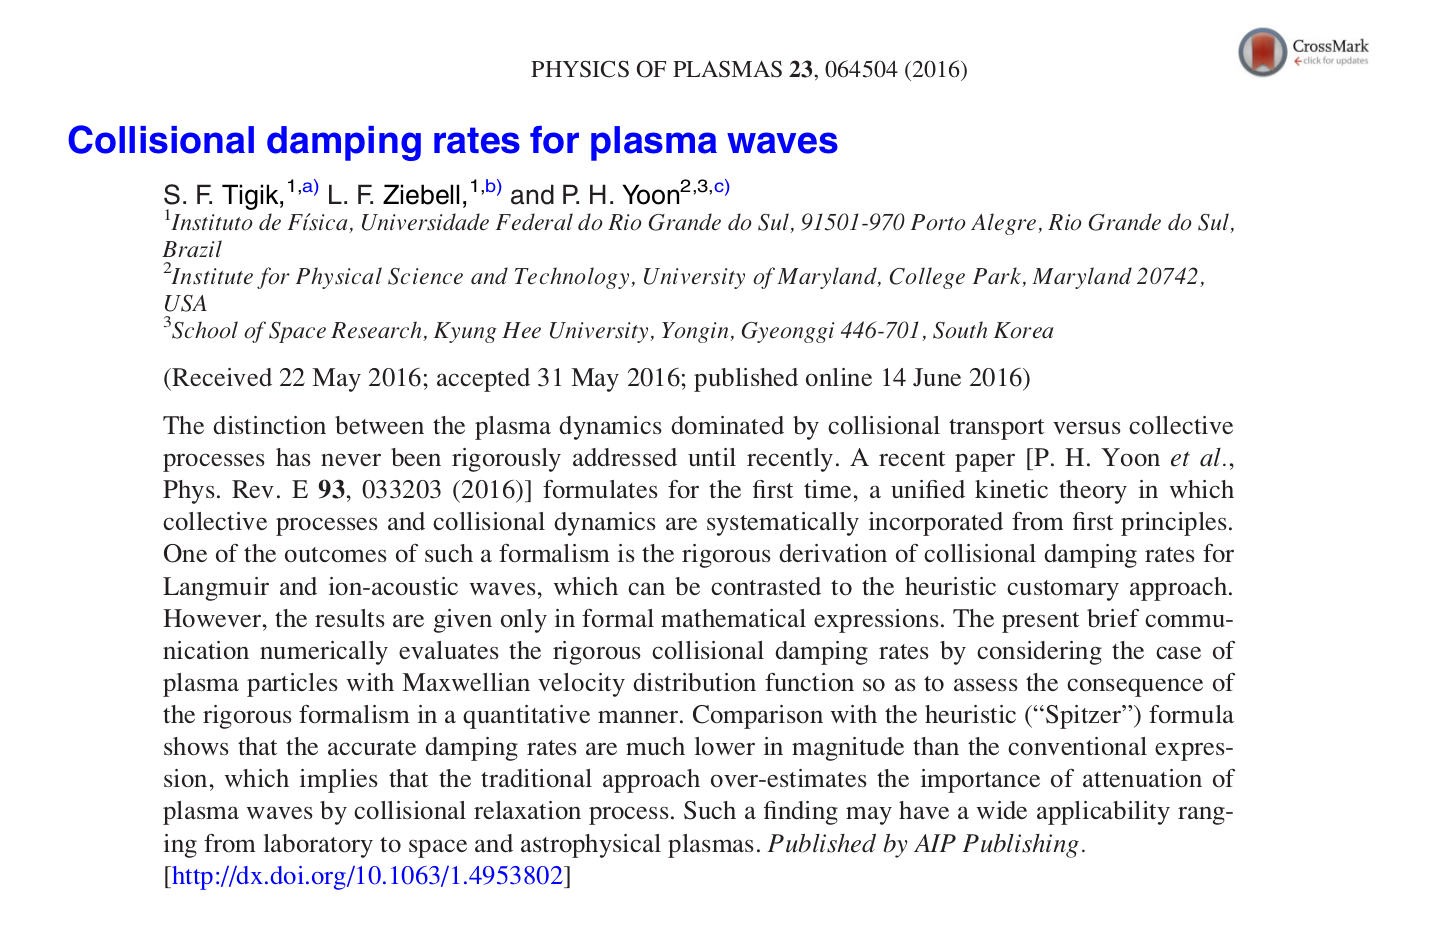
\includegraphics[width=0.9\textwidth]{print_Tigik2016b.png}
\end{frame}

\subsection*{Objetivos}
\begin{frame}
  \frametitle{Objetivos do estudo}
  \begin{itemize}
    \item Na modelagem de dados observacionais, quando há evidências
    de que colisões possam fazer parte da dinâmica, normalmente
    inclui-se um termo de colisões na equação das partículas e um
    termo de amortecimento colisional na equação das ondas;
    \vspace{0.1cm}
    \pause
    \item O termo de amortecimento colisional é, por via de regra,
    uma expressão constante, adicionada à equação das ondas de
    maneira \emph{ad hoc}, conhecida como fórmula de \emph{Spitzer}:
    \begin{displaymath}
      \gamma_{\mbox{\tiny coll}}=-\frac{\pi\, n_e e^4\,\ln \Lambda}{m_e^2v_{Te}^3},
    \end{displaymath}
    onde $\Lambda = 4\pi\,n_e\lambda_{De}^3$ e
    $\lambda_{De}=\sqrt{T_e/(4 \pi\, n_ee^2)}$;
    \vspace{0.1cm}
    \pause
    \item Neste estudo testamos a equivalência na intensidade do
    amortecimento colisional calculado com a nova equação de
    primeiros princípios com a intensidade calculada pela fórmula
    de Spitzer;
    \vspace{0.1cm}
    \pause
    \item Além disso, comparamos a taxa de amortecimento colisional
    com a taxa de amortecimento não colisional, considerando um
    plasma Maxwelliano.
  \end{itemize}
\end{frame}

\subsection*{Métodos}
\begin{frame}
  \frametitle{Normalização}
  \begin{itemize}
    \item Para a facilitar a análise numérica escrevemos as equações
    em termos das seguintes variáveis adimensionais
    \begin{displaymath}
      {\bf u}=\frac{\bf v}{v_{te}},\quad z_{\bf q}^\alpha
      =\frac{\omega_{\bf k}^\alpha}{\omega_{pe}},\quad
      {\bf q}=\frac{{\bf k}\,v_{te}}{\omega_{pe}}
      ={\bf k}\sqrt{2}\,\lambda_{De};
    \end{displaymath}
    \item Obtendo
    \begin{equation*}
      \label{GqL}
      \begin{split}
	\gamma_{\bf q}^{L\mbox{\tiny (coll)}}
	&= \frac{2gz_{\bf q}^L}{q^2}\int
	d{\bf q}' \frac{({\bf q}\cdot {\bf q'})^2}{{q'}^4
	  |\epsilon({\bf q'},z_{\bf q}^L)|^2}\left(1+\frac{T_e}{T_i}
	  +\frac{({\bf q}-{\bf q'})^2}{2}\right)^{-2}\\
	&\times\int d{\bf u}\,{\bf q'}\cdot
	\frac{\partial \Phi_e({\bf u})}{\partial {\bf u}}
	\delta(z_{\bf q}^L-{\bf q'}\cdot{\bf u}),
      \end{split}
    \end{equation*}
    \vspace{0.2cm}
    \begin{equation*}
      \label{GqS}
      \begin{split}
	\gamma_{\bf q}^{S\mbox{\tiny(coll)}}
	&=\frac{2g z_{\bf q}^L}{q^2}
	\int\frac{d{\bf q}'}{{q'}^4|\epsilon({\bf q'},z_{\bf q}^S)|^2}
	\left(1+\frac{T_e}{T_i}+\frac{({\bf q}-{\bf q'})^2}{2}\right)^{-2}
	\left(1+\frac{2T_e}{T_i}\frac{{\bf q}\cdot{\bf q}'}{q^2}\right)\\
	&\times \int d{\bf u}\, {\bf q'}\cdot\frac{\partial}{\partial {\bf u}}
	\left(\Phi_e({\bf u})+\frac{m_e}{m_i} \Phi_i({\bf u})\right)
	\delta(z_{\bf q}^S -{\bf q'}\cdot{\bf u}).
      \end{split}
    \end{equation*}
  \end{itemize}
\end{frame}


\begin{frame}
  \frametitle{Normalização}
  \begin{itemize}
    \item Em $\gamma_{\bf q}^{L\mbox{\tiny(coll)}}$ e em
    $\gamma_{\bf q}^{S\mbox{\tiny(coll)}}$, temos as seguintes
    quantidades
    \begin{eqnarray*}
      g=\frac{1}{2^{3/2}(4\pi)^2\hat n\,\lambda_{De}^3}
      =\frac{1}{2^{3/2}(4\pi\Lambda)},\qquad
      z_{\bf q}^L=1+\frac{3q^2}{4},\qquad
      z_{\bf q}^S=q \sqrt{\frac{m_e}{m_i}}\frac{1+3T_i/T_e}{2+q^2};
    \end{eqnarray*}
    \vspace{0.3cm}
    \item A normalização da fórmula de Spitzer é dada por
    \begin{displaymath}
      \bar \gamma_{\mbox{\tiny coll}}\equiv
      \frac{\gamma_{\mbox{\tiny coll}}}{\omega_{pe}}
      =-\frac{\pi\, n_ee^4\,\ln \Lambda}{m_e^2 v_{Te}^3\omega_{pe}}
      =- \pi g \ln \left( \frac{1}{2^{3/2}(4\pi g)} \right).
    \end{displaymath}
  \end{itemize}
\end{frame}

\begin{frame}
  \frametitle{Análise numérica}
  \begin{itemize}
    \item As equações para o amortecimento colisional das ondas $L$
    e $S$ foram integradas numericamente, considerando um plasma
    Maxwelliano e parâmetro de plasma $g=5\times 10^{-3}$;
    \vspace{0.25cm}
    \pause
    \item Nessa primeira análise, as novas equações não foram
    incluídas na subrotina de evolução temporal do programa
    principal;
    \vspace{0.25cm}
    \pause
    \item A fórmula de Spitzer, bem mais simples, não tem
    dependência com o número de onda;\vspace{0.25cm}
    \pause
    \item Então, para fins de comparação, consideramos quatro
    valores distintos para o parâmetro de plasma $g$ e, com
    isso, calculamos quatro valores diferentes usando
    $\bar \gamma_{\mbox{\tiny coll}}/g
    = \pi \ln \left[2^{3/2}(4\pi g)\right]$.
  \end{itemize}
\end{frame}

\begin{frame}
  \frametitle{Amortecimento de Landau}
  \begin{itemize}
    \item Para compararmos os resultados das novas equações com
    um processo equivalente e bem conhecido, integramos também as
    expressões para o amortecimento de Landau das ondas $L$ e $S$:
    \begin{align*}
       \gamma_{\bf q}^L
      &= -\frac{\pi^{1/2}(z_{\bf q}^L)^2}{q^3}
	  \exp\left(-\frac{(z_{\bf q}^L)^2}{q^2}\right),\\
      \gamma_{\bf q}^S
      &= -\frac{\pi^{1/2}\mu_{\bf q}z_{\bf q}^Lz_{\bf q}^S}{q^3}
	  \sum_{a=e,i}\frac{T_e}{T_a}\left(\frac{m_a}{m_e}
	  \frac{T_e}{T_a}\right)^{1/2}\exp\left(-\frac{m_a}{m_e}
	  \frac{T_e}{T_a}\frac{(z_{\bf q}^S)^2}{q^2}\right).
    \end{align*}
    \vspace{0.2cm}
    \pause
    \item Os dados de cada modo de oscilação foram comparados
    graficamente, sobrepondo na mesma figura
    $\gamma_{\bf q}^{\alpha \mbox{\tiny(coll)}}/g$ e $\gamma_{\bf q}^\alpha$,
    para seus respectivos $\alpha=L$ e $\alpha=S$.
  \end{itemize}
\end{frame}

\subsection*{Resultados}
\begin{frame}
  \frametitle{Resultados para a fórmula de Spitzer}
  \begin{itemize}
    \item A taxa de amortecimento colisional dada pela fórmula de
    Spitzer, aplicável apenas para ondas $L$, foi calculada para os
    seguintes  valores de $g$:
    \begin{align*}
      g&=10^{-10}\quad \longrightarrow \quad
      \bar \gamma_{\mbox{\tiny coll}}/g \sim -61.12\\
      g&=10^{-8}\,\,\quad \longrightarrow \quad
      \bar \gamma_{\mbox{\tiny coll}}/g \sim -46.65\\
      g&=10^{-6}\,\,\quad \longrightarrow \quad
      \bar \gamma_{\mbox{\tiny coll}}/g \sim -32.18\\
      g&=10^{-4}\,\,\quad \longrightarrow \quad
      \bar \gamma_{\mbox{\tiny coll}}/g \sim -17.72\\
    \end{align*}
  \end{itemize}
\end{frame}

\begin{frame}
  \frametitle{Resultados da integração para ondas $L$}
  \begin{figure}
    \centering
    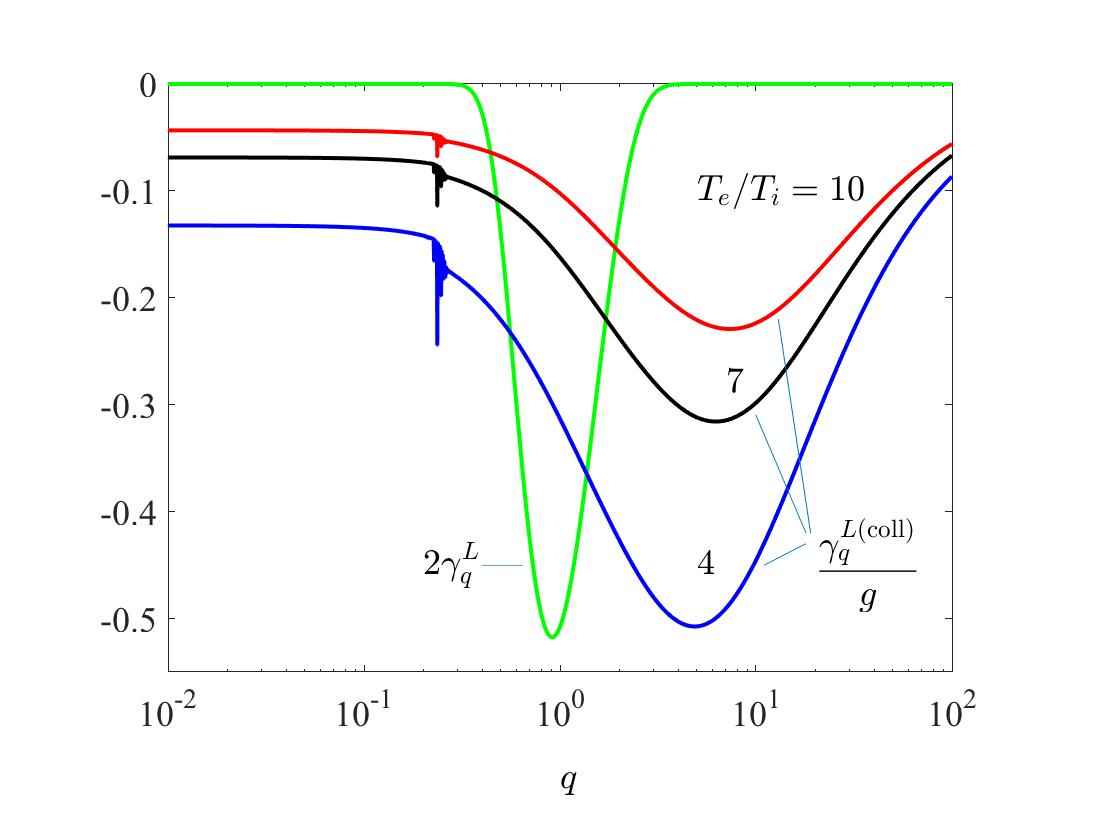
\includegraphics[width=0.65\textwidth]{F1}
    \caption*{Resultados para  $\gamma_{\bf q}^{L \mbox{\tiny(coll)}}/g$
      e $\gamma_{\bf q}^L$, considerando três temperaturas diferentes e
      $g=5\times 10^{-3}$.}
  \end{figure}
\end{frame}

\begin{frame}
  \frametitle{Resultados da integração para ondas $S$}
  \begin{figure}
    \centering
    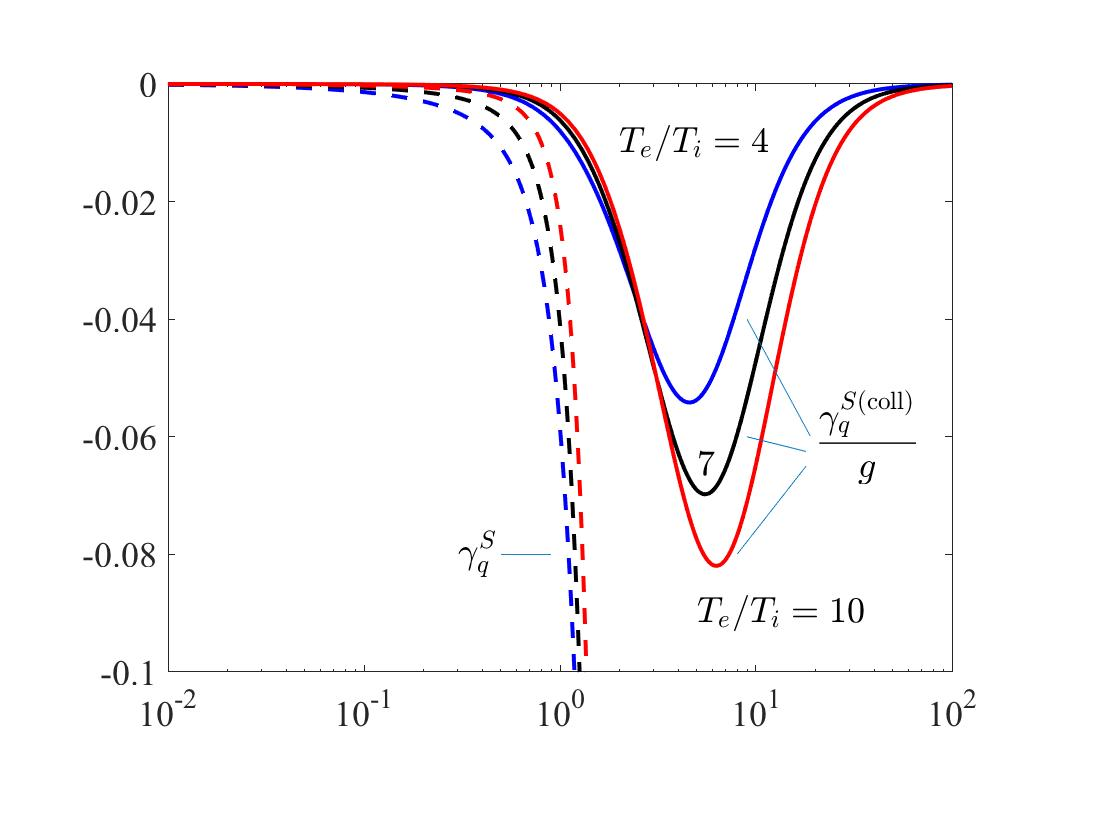
\includegraphics[width=0.65\textwidth]{F2}
    \caption*{Resultados para  $\gamma_{\bf q}^{S \mbox{\tiny(coll)}}/g$
      e $\gamma_{\bf q}^S$, considerando três temperaturas diferentes e
    $g=5\times 10^{-3}$.}
  \end{figure}
\end{frame}

\begin{frame}
  \frametitle{Conclusões a respeito desta análise}
  \begin{itemize}
    \item A taxa de amortecimento colisional, em comparação com
    a taxa de amortecimento não colisional, é praticamente desprezível;
    \vspace{0.4cm}
    \pause
    \item Lembrando que, nas figuras, $\gamma_{\bf q}^{\alpha \mbox{\tiny(coll)}}$
    está dividido por  $g=5\times 10^{-3}$, enquanto $\gamma_{\bf q}^\alpha$ não;
    \vspace{0.4cm}
    \pause
    \item Quando comparamos o resultado da integração da expressão formal
    para o amortecimento colisional, com os valores calculados com a
    fórmula de Spitzer, os valores divergem por, pelo menos, seis ordens
    de grandeza;
    \vspace{0.4cm}
    \pause
    \item Esse resultado sugere que o amortecimento colisional
    vem sendo superestimado na modelagem de dados observacionais;
    \vspace{0.4cm}
    \pause
    \item O que põe em evidência a importância de uma teoria de primeiros
    princípios que combine processos coletivos e interações colisionais.
  \end{itemize}
\end{frame}

\section*{Geração de elétrons supratérmicos por processos
  coletivos em plasmas colisionais}
% \subsection{Geração de elétrons supratérmicos por processos
%   coletivos em plasmas colisionais}
\begin{frame}
  \frametitle{Geração de elétrons supratérmicos e o processo de
    bremsstrahlung eletrostático}
 \centering 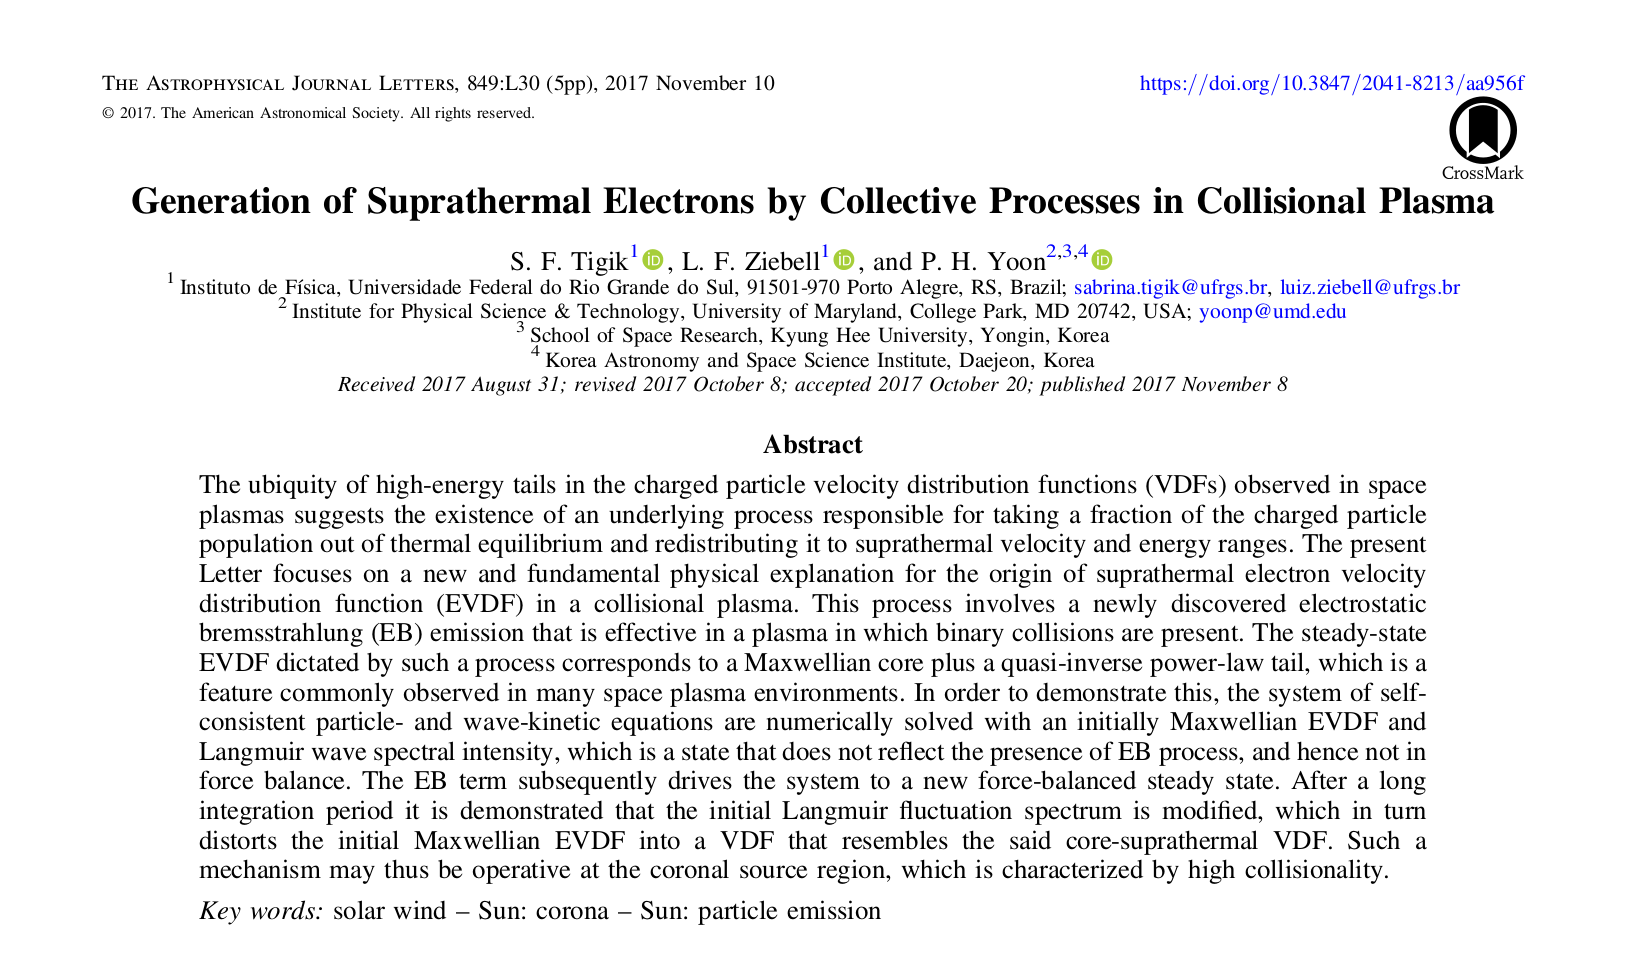
\includegraphics[width=0.9\textwidth]{print_Tigik2017a.png}
\end{frame}

\subsection*{Objetivos}
\begin{frame}
  \frametitle{Objetivos do estudo}
  \begin{itemize}
    \item Ao contrário do amortecimento colisional, o bremsstrahlung
    eletrostático não possui um processo equivalente com o qual pudesse
    se comparado;
    \vspace{0.5cm}
    \item Portanto, o principal objetivo deste estudo foi analisar
    como o efeito de bremsstrahlung eletrostático afeta a evolução
    temporal do plasma e tentar entender fisicamente como isso
    acontece.
  \end{itemize}
\end{frame}

\subsection*{Métodos}
\begin{frame}
  \frametitle{Configuração do sistema}
  \begin{itemize}
    \item Para evidenciar a atuação do bremsstrahlung eletrostático,
    consideramos o sistema mais simples possível;
    \vspace{0.4cm}
    \pause
    \item Um plasma Maxwelliano que evolui de acordo com o formalismo
    quaselinear, que inclui emissão espontânea e difusão no espaço
    de velocidades.
    \vspace{0.4cm}
    \pause
    \item Nessa configuração, com uma função de distribuição monotonicamente
    decrescente como a Maxwelliana, esperávamos que nada fosse acontecer e
    então partiríamos para uma análise com a instabilidade \emph{bump-in-tail};
    \vspace{0.4cm}
    \pause
    \item Só que não foi bem assim, como veremos em seguida;
    \vspace{0.4cm}
    \pause
    \item Então, pela natureza das modificações ocorridas na função de
    distribuição, decidimos que seria interessante incluir também os
    efeitos de colisões binárias.
  \end{itemize}
\end{frame}

\begin{frame}
  \frametitle{Equações adimensionais}
  \begin{itemize}
    \item As variáveis adimensionais são as mesmas, mas nesse
    caso precisamos normalizar também as equações cinéticas das
    partículas e das ondas e o tempo:
    \begin{align*}
      \Phi_a({\bf u})=  v_e^3 F_a({\bf u}),
      \quad {\cal E}_{\bf q}^{\sigma\alpha}
      = \frac{(2\pi)^2 g}{m_ev_e^2}
      \frac{I_{\bf k}^{\sigma\alpha}}{\mu_{\bf k}^\alpha},
      \quad  P_{\bf k}^\alpha=\frac{m_ev_e^2}{(2\pi)^2g}
      \omega_{pe}P_{\bf q}^\alpha,
      \quad \tau = \omega_{pe}t;
    \end{align*}
    \item A equação cinética normalizada para as ondas $L$ é a
    seguinte
    \begin{equation*}
      \begin{split}
	\frac{\partial{\cal E}_{\bf q}^{\sigma L}}{\partial\tau}
	&=\mu_{\bf q}^L\,\frac{\pi}{q^2}\int d{\bf u}\;
	\delta(\sigma z_{\bf q}^L-{\bf q}\cdot{\bf u})\\
	&\times\biggl(g\,\Phi_e({\bf u})+(\sigma z_{\bf q}^L)
	{\bf q}\cdot\frac{\partial \Phi_e({\bf u})}{\partial{\bf u}}
	{\cal E}_{\bf q}^{\sigma L}\biggr) +2{\cal E}_{\bf q}^{\sigma L}
	\gamma_{\bf q}^{\sigma L}+P_{\bf q}^{\sigma L};
      \end{split}
    \end{equation*}
    \item Neste trabalho não analisamos o espectro das ondas $S$.
  \end{itemize}
\end{frame}

\begin{frame}
  \frametitle{Equação adimensional para o bremsstrahlung
    eletrostático}
  \begin{itemize}
    \item As expressões normalizadas para o bremsstrahlung são dadas por
    \begin{equation*}
      \begin{split}
	P_{\bf q}^{\sigma L} &= \frac{12e^2}{\pi^3}
	\frac{1}{q^2}\frac{1}{(z_{\bf q}^L)^2}
	\left(1-\frac{m_e}{m_i}\frac{T_e}{T_i}\right)^2
	\frac{\omega_{pe}^2}{v_e}\int d{\bf q'}\,q'^2|{\bf q-q'}|^2\\
	&\times \left[2\left(1+\frac{T_e}{T_i}\right)+q'^2\right]^{-2}
	\left[2\left(1+\frac{T_e}{T_i}\right) +|{\bf q-q'}|^2\right]^{-2}\\
	&\times \int d{\bf u}\int d{\bf u'} \delta \left[ \sigma
	  z_{\bf q}^L-{\bf q\cdot u} +{\bf q'}\cdot ({\bf u-u'})\right]
	\sum_a \Phi_a({\bf u})\sum_b \Phi_b({\bf u'}).
      \end{split}
    \end{equation*}
  \end{itemize}
\end{frame}

\begin{frame}
  \frametitle{Forma adimensional da equação cinética das partículas
    e do operador colisional}
  \begin{itemize}
    \item Para a equação cinética adimensional para as partículas, temos
    \begin{equation*}
      \begin{split}
	\frac{\partial \Phi_a({\bf u})}{\partial \tau}
	&=\frac{e_a^2}{e^2}\frac{m_e^2}{m_a^2}
	\sum_\sigma\sum_{\alpha=L,S}\int d{\bf q}\;\biggl(
	\frac{\bf q}{q} \cdot\frac{\partial}{\partial{\bf u}}
	\biggr)\,\mu_{\bf q}^\alpha\;\delta(\sigma z_{\bf q}^\alpha
	-{\bf q}\cdot{\bf u})\\
	&\times\,\biggl(g\frac{m_a}{m_e}\frac{\sigma z_{\bf q}^L}{q}\,
	\Phi_a({\bf u})+{\cal E}_{\bf q}^{\sigma\alpha}\;\frac{\bf q}{q}
	\cdot\frac{\partial \Phi_a({\bf u})}{\partial{\bf u}}\biggr)
	+\sum_b\theta_{ab}(\Phi_a,\Phi_b);
      \end{split}
    \end{equation*}\vspace{-0.4cm}
    \pause
    \item Por fim, a forma adimensional do operador colisional de Landau
    linearizado
    \begin{equation*}
      \begin{split}
	\theta_{ab}(\Phi_a,\Phi_b) &= \Gamma_{ab}\left\{
	  \frac{\partial}{\partial{\bf u}_a}\cdot
	  \left(2\frac{m_a}{m_b}\Psi(u_{ab})
	    \frac{{\bf u}_a}{u^3_a}\Phi_a\right)\right.\\
	&+\frac{\partial}{\partial{\bf u}_a}\cdot
	 \left\{\left[\left(\Phi(u_{ab})
	      -\frac{1}{2 u_{ab}^2}\Psi(u_{ab})\right)
	    \frac{\partial^2u_a}{\partial{\bf u}_a
	      \partial{\bf u}_a}\right]\cdot
	  \frac{\partial \Phi_a}{\partial{\bf u}_a}\right\}\\
	&+\left. \frac{\partial}{\partial{\bf u}_a}\cdot
        \left[\left(\frac{1}{u_{ab}^2}\Psi(u_{ab})
	      \frac{{\bf u}_a{\bf u}_a}{u_a^3}\right)\cdot
	    \frac{\partial \Phi_a}{\partial{\bf u}_a}\right]\right\},
      \end{split}
    \end{equation*}
    onde  $u_{ab}\equiv u_a (v_{T_a}/v_{T_b})$ e
    $\Gamma_{ab}=2\pi g Z_b^2 \ln\Lambda $, sendo
    $g=1/[2^{3/2}(4\pi)^2\hat n \lambda_{De}^3]$.
  \end{itemize}
\end{frame}

\begin{frame}
  \frametitle{Condições iniciais}
  \begin{itemize}
    \item As funções de distribuição iniciais para os íons e para os
    elétrons são Maxwellianas
    \begin{displaymath}
      F_a({\bf v})=\frac{1}{\pi^{3/2}v_a^3}
      \exp \left(-\frac{v^2}{v_a^2}\right),
    \end{displaymath}
    onde $v_a=(2T_a/m_a)^{1/2}$;
    \vspace{0.1cm}
    \pause
    \item Durante a evolução temporal os íons permanecem estáticos,
    enquanto a função de distribuição dos elétrons evolui;
    \vspace{0.1cm}
    \pause
    \item A razão de temperatura entre íons e elétrons foi
    definida com sendo $T_e/T_i=7$;
    \vspace{0.1cm}
    \pause
    \item O parâmetro de plasma escolhido foi
    $g=1/(n_e\lambda_{De}^3)=5\times 10^{-3}$;
    \vspace{0.1cm}
    \pause
    \item A condição inicial das ondas de Langmuir foi
    obtida balanceando os efeitos de emissão induzida e
    emissão espontânea, obtendo a seguinte expressão
    \begin{displaymath}
      I_{\bf k}^{\sigma L}(0)=\frac{T_e}{4\pi^2}
      \left( 1+3k^2\lambda_{De}^2\right).
    \end{displaymath}
  \end{itemize}
\end{frame}

\begin{frame}
  \frametitle{Análise numérica}
  \begin{itemize}
    \item O sistema de equações íntegro-diferenciais foi integrado
    em duas dimensões;
    \vspace{0.3cm}
    \pause
    \item Foi escrita uma subrotina de integração para o termo
    de bremsstrahlung eletrostático;
    \vspace{0.3cm}
    \pause
    \item A equação das partículas, foi escrita na forma de diferenças
    finitas e integrada usando o método \emph{splitting}, com passo de
    tempo fixo;
    \vspace{0.3cm}
    \pause
    \item A equação das ondas, foi integrada usando o método Runge-Kutta
    de quarta ordem.
  \end{itemize}
\end{frame}

\subsection*{Resultados}
\begin{frame}
  \frametitle{Resultado para a evolução do espectro das
  ondas $L$}
  \begin{figure}
    \centering
    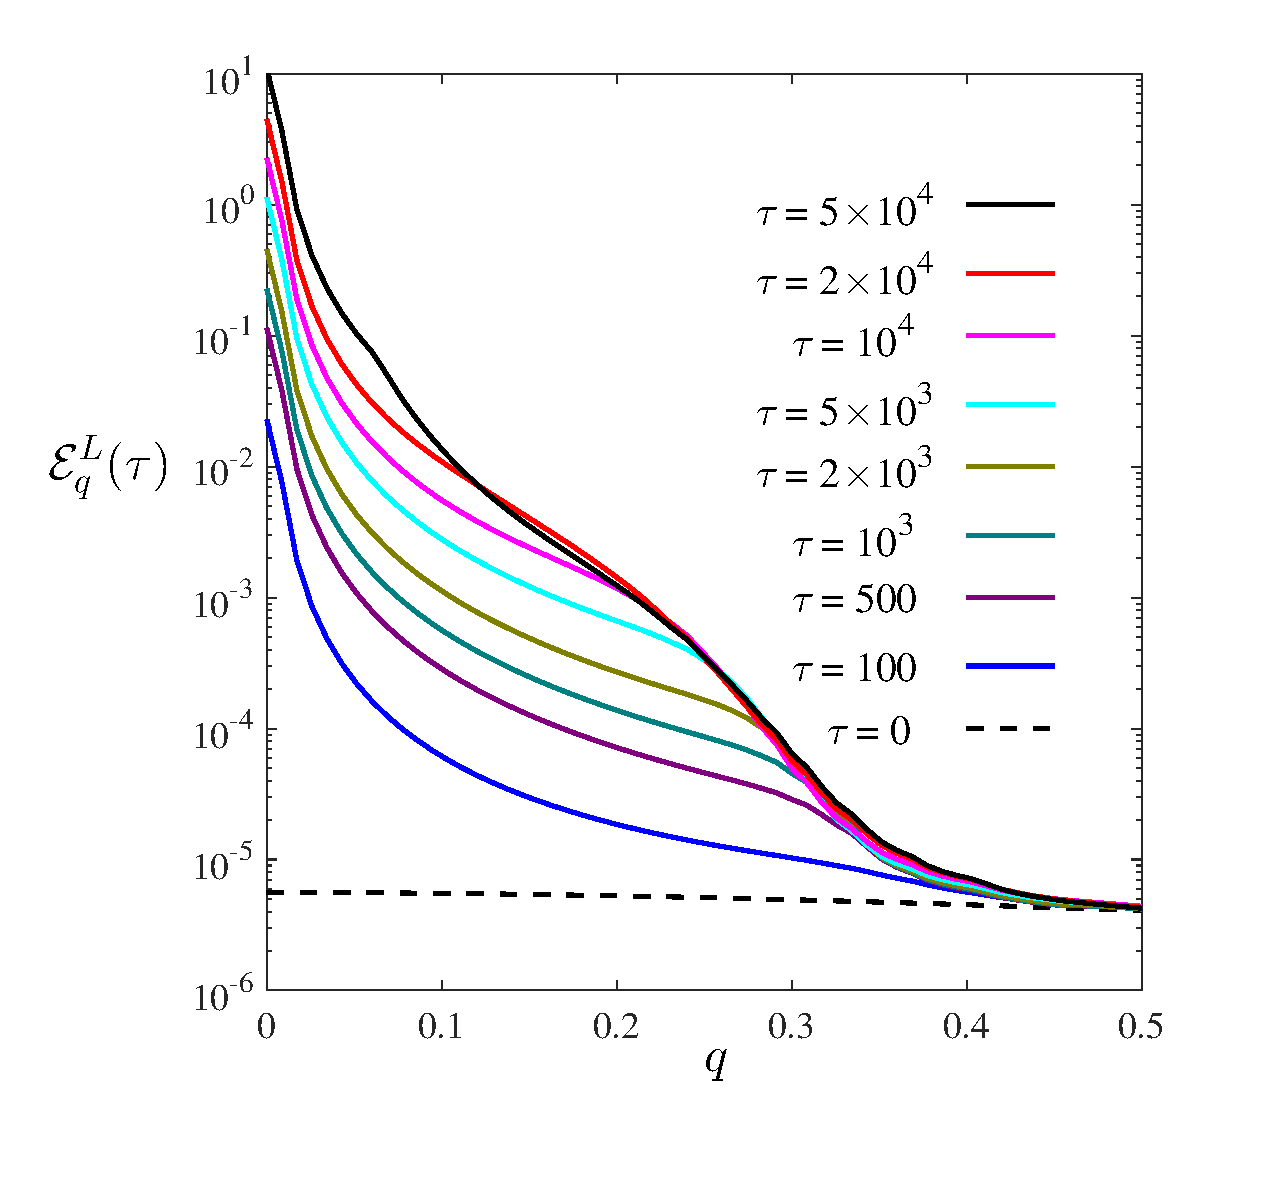
\includegraphics[width=0.6\textwidth]{Figure1}
    \caption*{Evolução temporal do espectro das ondas de Langmuir.}
  \end{figure}
\end{frame}

\begin{frame}
  \frametitle{Resultado para a função de distribuição de
  velocidades}
  \begin{figure}
    \centering
    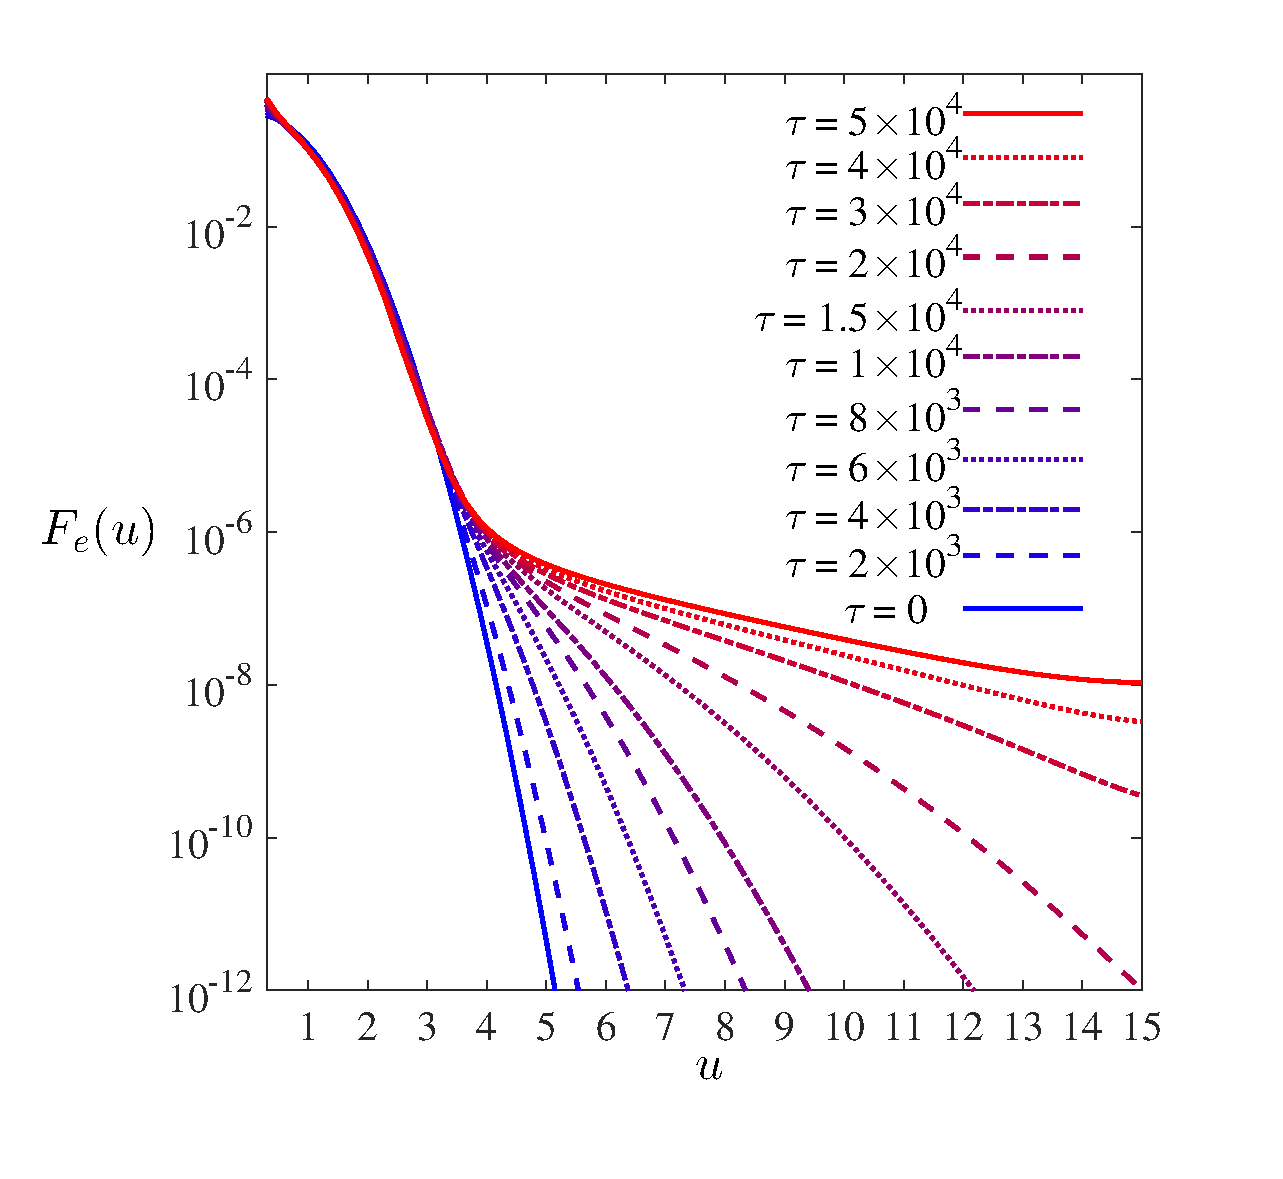
\includegraphics[width=0.6\textwidth]{Figure2}
    \caption*{Evolução temporal da função de distribuição de velocidades
    dos elétrons.}
  \end{figure}
\end{frame}

\begin{frame}
  \frametitle{Por que este resultado é interessante?}
  \begin{itemize}
    \item Distribuições supratérmicas, tanto de elétrons quanto de prótons,
    são pervasivas em plasmas espaciais;
    \vspace{0.1cm}
    \pause
    \item Elas são observadas em uma enorme variedade de ambientes e sob
    diferentes condições;
    \vspace{0.1cm}
    \pause
    \item O que sugere que essas distribuições têm origem em algum
    processo fundamental, inerente à dinâmica das partículas carregadas
    e não das condições no entorno dessas partículas;
    \vspace{0.1cm}
    \pause
    \item Sendo necessário apenas um certo grau de ionização para que
    esse processo comece a atuar no sistema;
    \vspace{0.1cm}
    \pause
    \item Esses dois últimos pontos são suposições, claro. Mas são suposições
    que merecem investigação;
    \vspace{0.1cm}
    \pause
    \item Há evidências de que essas distribuições supratérmicas alteram a dinâmica
    do plasma e podem participar de processos que ainda não são totalmente
    compreendidos, como, por exemplo, a inversão de temperatura observada na coroa
    solar.
  \end{itemize}
\end{frame}

\section*{Estado assintótico}
\begin{frame}\frametitle{Equação para o estado assintótico das ondas $L$}
  \begin{itemize}
  \item A equação para o estado assintótico das ondas $\alpha$,
    incluindo os novos efeitos, é dada por
  \end{itemize}
  \begin{equation}
    {\cal E}_{\bf q}^{\sigma {\alpha}}(0)
    =-\frac{S_{\bf q}^{\alpha} + P_{\bf q}^{\alpha}}{\hspace{0.60cm}\gamma_{\bf q}^{\alpha} 
  +2\gamma_{\bf q}^{{\alpha}\mbox{\tiny (coll)}}}.
  \end{equation}
\end{frame}

\begin{frame}
  \frametitle{Estados assintóticos com bremsstrahlung
  eletrostático}
  \begin{figure}
    \centering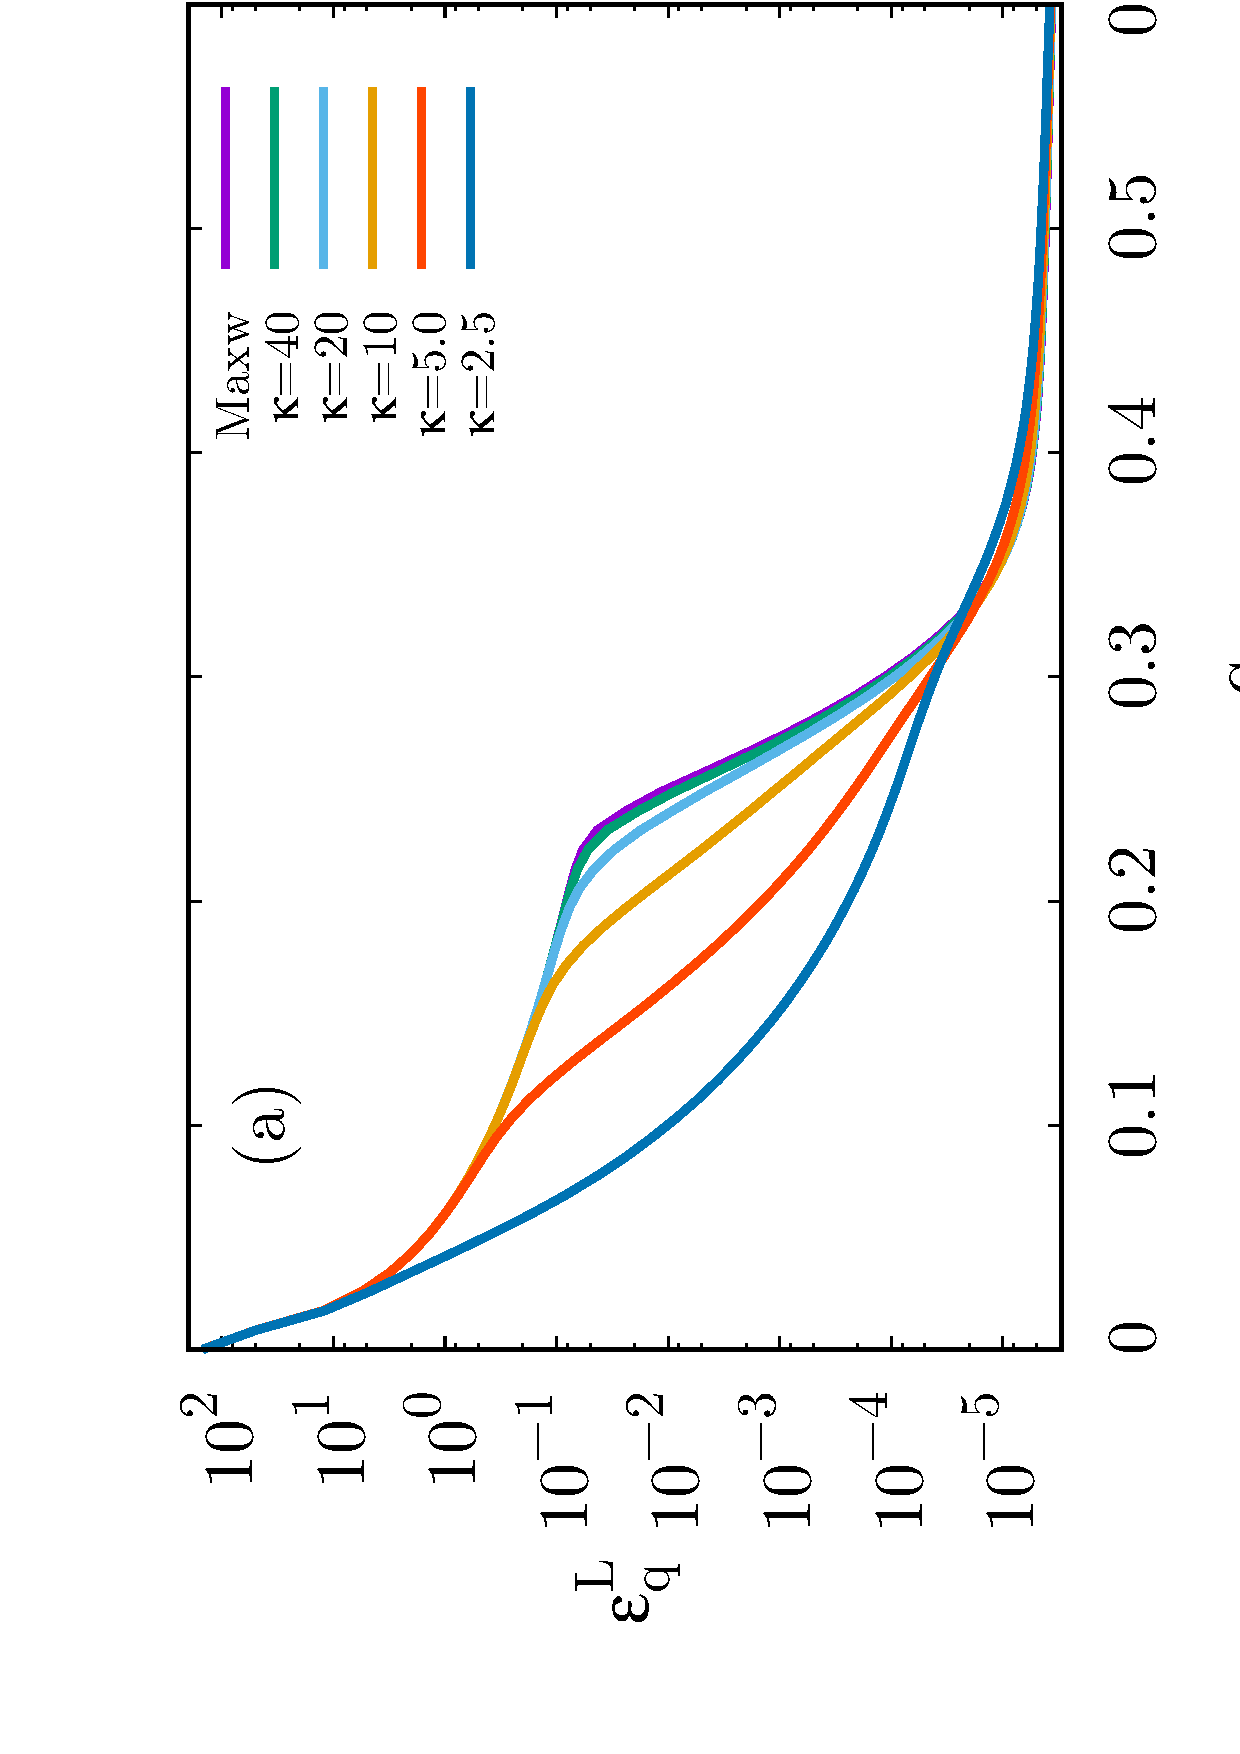
\includegraphics[width=0.5\textwidth,angle=270]{IL1D_005kvar}
    \caption*{Estado assintótico do espectro das ondas de Langmuir com o
      efeito de bremsstrahlung eletrostático incluído, para uma função de
      distribuição Maxwelliana e para diversos índices $\kappa$.}
  \end{figure}
\end{frame}


\begin{frame}
  \frametitle{Estados assintóticos sem bremsstrahlung
    eletrostático}
  \begin{figure}
    \centering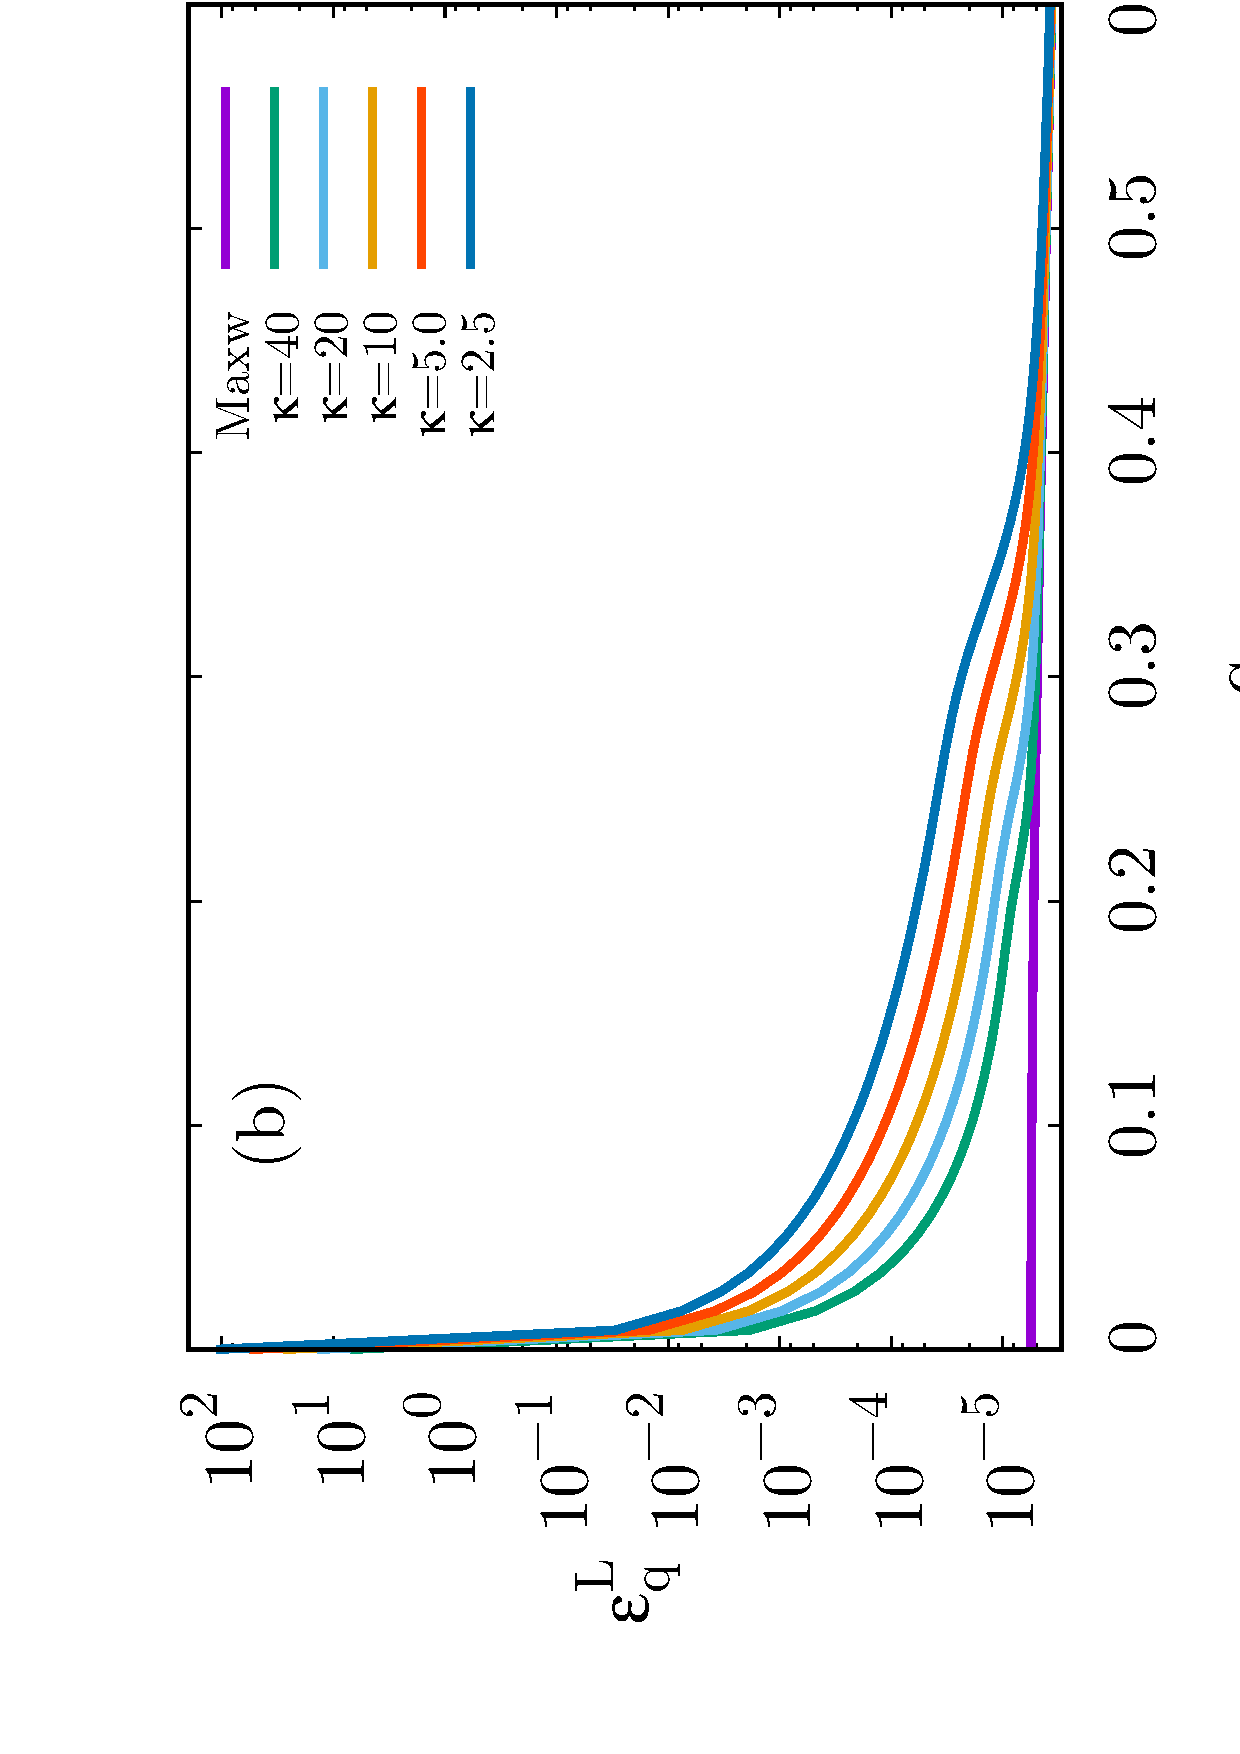
\includegraphics[width=0.5\textwidth,angle=270]{IL1D_005kvarno-brem}
    \caption*{Estado assintótico do espectro das ondas de Langmuir sem o
      efeito de bremsstrahlung eletrostático incluído, para uma função de
      distribuição Maxwelliana e para diversos índices $\kappa$.}
  \end{figure}
\end{frame}



\section{Publicação extra}
\begin{frame}
  \frametitle{Processos fracamente turbulentos na presença de
    uma população supratérmica}
   \centering 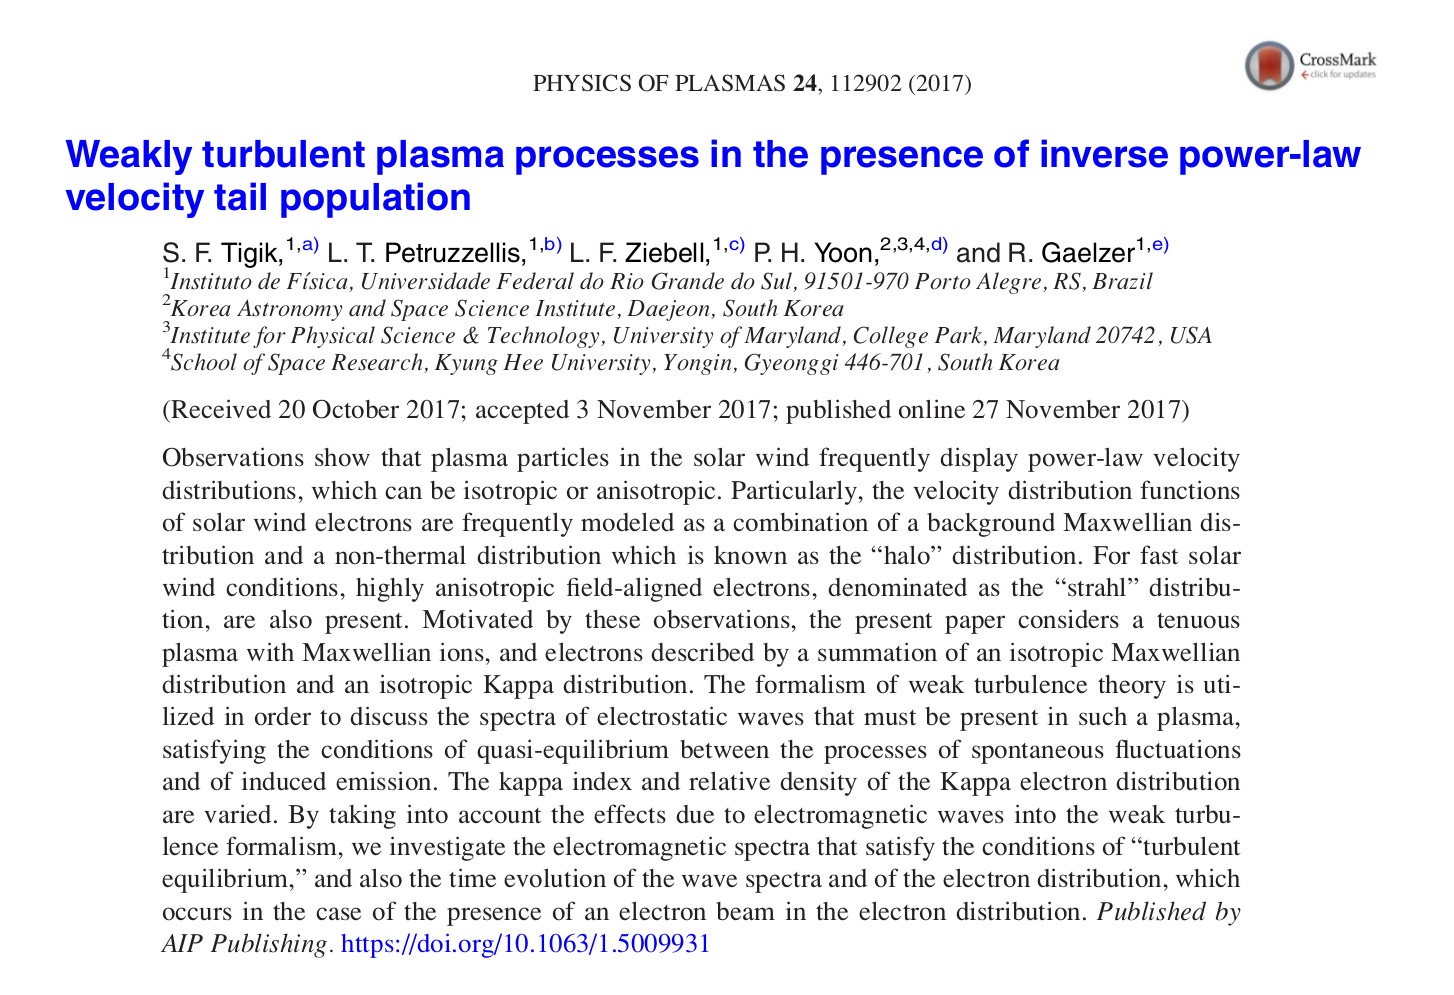
\includegraphics[width=0.9\textwidth]{print_Tigik2017b.png}
\end{frame}

\begin{frame}
  \frametitle{Sobre este trabalho}
  \begin{itemize}
    \item Este trabalho envolve a análise do espectro das oscilações
    eletromagnéticas, em um plasma não magnetizado, na presença de uma
    função de distribuição com núcleo Maxwelliano e um \emph{halo} de
    elétrons supratérmicos, modelados por uma função de distribuição
    do tipo $\kappa$;
    \vspace{0.2cm}
    \pause
    \item A análise é feita com o uso da teoria de turbulência fraca,
    e o processo de integração é, basicamente, o mesmo;
    \vspace{0.2cm}
    \pause
    \item Contudo, este trabalho não envolve nenhum tipo de interação
      colisional, enquanto o estudo apresentado até o momento considera
      apenas ondas eletrostáticas e função de distribuição Maxwelliana;
    \vspace{0.2cm}
    \pause
    \item Os resultados deste trabalho mostram que, mesmo a presença de
    uma pequena população supratérmica na função de distribuição de
    velocidades dos elétrons, é capaz de alterar o espectro assintótico
    tanto das ondas transversais  $(T)$, quanto das ondas de Langmuir.
  \end{itemize}
\end{frame}

\section*{Entre a entrega da tese e a defesa um artigo foi aceito}
% \subsection*{\emph{Bremsstrahlung} eletrostático e amortecimento
%   colisional como processos inversos}
\begin{frame}
  \frametitle{Emissão de \emph{bremsstrahlung} e amortecimento colisional
    para ondas de Langmuir}
  \begin{figure}
    \centering \includegraphics[width=0.82\textwidth]{print_Tigik2019.png}
   \caption*{Artigo Submetido à revista \emph{Plasma Physics and Controlled
      Fusion (PPCF)}.}
  \end{figure}
\end{frame}

\begin{frame}
  \frametitle{Processos inversos}
  \begin{itemize}
  \item As equações para a emissão de \emph{bremsstrahulng} eletrostático
    e para o amortecimento colisional são processos inversos na 
  \end{itemize}
\end{frame}

\begin{frame}
  \frametitle{Fim}
  \vspace{1.2cm}
  \centering {\Huge{\bf Obrigada!}} %$\bigstar$

  \vspace{1.2cm}

  \begin{figure}
    \caption*{Financiamento:}
    \centering
    
\includegraphics[width=0.22\textwidth]{cnpq.png}
    \hspace{1cm} \includegraphics[width=0.13\textwidth]{capes.png}
  \end{figure}
\end{frame}

\begin{frame}[noframenumbering]
  \frametitle{Equações microscópicas de Klimontovich}
  %\framesubtitle{}
  \begin{itemize}
\item Vamos considerar novamente ondas eletrostáticas e a ausência de campos
  externos;
\item Tomando a média das equações microscópicas do formalismo de Klimontovich,
  temos
  \begin{eqnarray}
  \left<N_a(x,t)\right>&=n_a f_a(x,t), \quad 
  \left<{\bf E}^M\right>&= {\bf E}({\bf r},t),
  \end{eqnarray}
  e a identidade $\left<{\bf E}^M N_a(x,t)\right> = {\bf E}({\bf r},t)n_af_a(x,t)
  + \left<{\delta \bf E}^M \delta N_a\right>_{{\bf r},x,t}$;
\item Disso obtemos o seguinte sistema de equações
  \begin{equation}
  \begin{split}
    \frac{\partial f_a}{\partial t}
    +{\bf v \cdot}\frac{\partial f_a}{\partial \bf r}
    +\frac{e_a}{m_a}{\bf E}{\bf \cdot}\frac{\partial f_a}{\partial \bf v}
    &=-\frac{e_a}{n_a m_a} \frac{\partial }{\partial \bf v}{\bf \cdot}
    \left<\delta{\bf E}\delta N_a\right>_{{\bf r},x,t}\equiv C_a(x,t),\\
    \nabla {\bf \cdot E}=4\pi& \sum_a e_a n_a \int d^3v\ f_a({\bf r,v},t),
  \end{split}
  \label{sist-av}
  \end{equation}
  \end{itemize}
\end{frame}

\begin{frame}[noframenumbering]
  \frametitle{Integral colisional}
  \begin{itemize}
  \item Temos ainda a equação de movimento para as flutuações aleatórias
  \begin{equation}
  %\begin{split}
    \frac{\partial \delta N_a}{\partial t}
    +{\bf v \cdot}\frac{\partial \delta N_a}{\partial \bf r}
    +\frac{e_a}{m_a}{\bf E \cdot} \frac{\partial\ \delta N_a}{\partial \bf v}
    +\frac{e_an_a}{m_a}\delta {\bf E \cdot} \frac{\partial f_a}{\partial \bf v}
    =-\frac{e_a}{m_a}\frac{\partial}{\partial \bf v}
    \cdot \bigl(\delta{\bf E}\delta N_a
    -\left<\delta{\bf E}\delta N_a\right>_{{\bf r},x,t} \bigr).
  %\end{split}
  \label{evol-flut}
  \end{equation}
\item Escrevendo o segundo momento em termos de
  $\left<\delta N_a \delta N_b\right>_{x,x',t}$ 
  \begin{equation}
  \left<\delta {\bf E} \delta N_a \right>_{{\bf r},x,t}
  =-\sum_b e_b \int dx'\ \frac{\partial}{\partial \bf r} \frac{1}{|{\bf r-r'}|}
  \left<\delta N_a \delta N_b \right>_{x,x',t}.
  \label{pot-ave}
  \end{equation}
\item Ficamos com a seguinte expressão para o termo de colisões
  \begin{equation}
  C_a(x,t)=\frac{1}{n_am_a}\sum_b\int d^3r'd^3v'\
  \frac{\partial}{\partial \bf r}\frac{e_ae_b}{\bf | r-r'|}
  \cdot\frac{\partial}{\partial \bf v}
  \left<\delta N_a({\bf r,v},t)\delta N_b({\bf r',v'},t)\right>.
  \label{c_a}
  \end{equation}
  \end{itemize}
\end{frame}

\begin{frame}[noframenumbering]
  \frametitle{Equações hierárquicas de Klimontovich}
  %\framesubtitle{}
  \begin{itemize}
\item Ao tentarmos escrever uma equação para a evolução do segundo momento central,
  chegamos à seguinte expressão
  \begin{equation}
  \begin{split}
    \frac{\partial }{\partial t}&\left<\delta N_a\delta N_b\right>_{x,x',t}
    +{\bf v \cdot}
    \frac{\partial }{\partial \bf r}\left<\delta N_a\delta N_b\right>_{x,x',t}
    +{\bf v' \cdot}
    \frac{\partial }{\partial \bf r'}\left<\delta N_a\delta N_b\right>_{x,x',t}\\
    &+\frac{e_a}{m_a}{\bf E}\cdot \frac{\partial }{\partial \bf v}
    \left<\delta N_a \delta N_b\right>_{x,x',t}
    +\frac{e_b}{m_b}{\bf E}\cdot\frac{\partial }{\partial \bf v'}
    \left<\delta N_a\delta N_b\right>_{x,x',t}\\
    &+\frac{e_an_a}{m_a}\left<\delta {\bf E} \delta N_b\right>_{{\bf r},x,t}
    \cdot\frac{\partial f_a}{\partial \bf v}
    +\frac{e_bn_b}{m_b}\left<\delta N_a\delta {\bf E}\right>_{x,{\bf r'},t}
    \cdot\frac{\partial f_b}{\partial \bf v'}\\
    =&-\frac{e_a}{m_a}\frac{\partial}{\partial \bf v}
    \cdot\left<\delta{\bf E}\delta N_a\delta N_b\right>_{{\bf r},x,x',t}
    -\frac{e_b}{m_b}\frac{\partial}{\partial \bf v'}
    \cdot \left<\delta N_a\delta{\bf E}\delta N_b\right>_{x',{\bf r},x',t},
  \end{split}
  \label{segunda}
  \end{equation}
\item onde $\delta {\bf E}$ é dado por
$ \nabla {\bf \cdot}\delta{\bf E}=4\pi \sum_a e_a \int d^3v\ \delta N_a$.
\item Vemos a equação (\ref{segunda}) mantém o sistema de equações aberto, devido a
  presença do terceiro momento no lado direito da igualdade.
  \end{itemize}
\end{frame}

\begin{frame}[noframenumbering]
  \frametitle{Parâmetro de plasma}
  %\framesubtitle{}
  \begin{itemize}
\item Precisamos truncar essa cadeia de equações, para isso, vamos definir um
  critério conhecido como parâmetro de plasma:
\item Em gases neutros e rarefeitos, a esfera de interação molecular
  tem um raio da ordem do raio das moléculas, $r_0 \sim \unit[10^{-8}-10^{-7}]{cm}$;
\item Isso torna a interação entre três ou mais moléculas algo muito raro;
\item Em plasmas, as interações entre as cargas são dominadas pela lei de Coulomb,
  de longo alcance, logo, a intensidade da interação decai lentamente;
\item Nesse caso, uma partícula interage ao mesmo tempo com muitas outras partículas
  e o alcance das interações efetivas entre as cargas é dado por
  $\lambda_D^2=T/(4\pi \sum_a e_a^2 n_a)$;
\item Na maioria dos plasmas, a esfera de Debye contém um grande número de
  partículas, isto é, $n\lambda_D^3 \gg 1$;
\item O parâmetro de plasma é definido como o inverso do número de partículas em uma
  esfera de Debye
  \begin{equation}
  g=\frac{1}{n\lambda_D^3}.
  \label{plasma-parameter}
  \end{equation}
  \end{itemize}
\end{frame}

\begin{frame}[noframenumbering]
  \frametitle{Parâmetro de plasma e correlações entre partículas}
  %\framesubtitle{}
  \begin{itemize}
\item Analisando as definições das quantidades $g$ e $\lambda_D$, vemos que
  $g$ é da mesma ordem da razão entre a energia média de interação entre duas
  partículas e a energia cinética de uma dessas partículas
  \begin{equation}
  g\sim \frac{e^2n^{1/3}}{T};
  \end{equation}
\item Se $g\ll 1$, isto é, a energia de interação é muito menor do que a energia
  cinética, podemos assumir que a correlação entre as partículas seja fraca;
\item Escrevendo o segundo momento central em termos da correlação de pares, temos
  \begin{equation}
  \left<\delta N_a(x,t) \delta N_b(x',t)\right>
  =n_an_b\ g_{ab}(x,x',t)+\delta_{ab}\delta(x-x')n_af_a;
  \label{pares}
  \end{equation}
\item Podemos supor que $f_a \sim {\cal O}(1),\ \,\,\,\, g_{ab}\sim {\cal O}(g),\
  \,\,\,\, g_{abc}\sim {\cal O}(g^2),\ ...$
  \end{itemize}
\end{frame}

\end{document}